%\documentclass[ART_main.tex]{subfiles}
\documentclass[ngerman, DIV=11, BCOR=0mm, paper=a4, fontsize=11pt, parskip=half, twoside=false, titlepage=true]{scrreprt}
%\graphicspath{ {Bilder/} {../Bilder/} }


\usepackage[singlespacing]{setspace}
\usepackage{lastpage}
\usepackage[automark, headsepline]{scrlayer-scrpage}
\clearscrheadings
\setlength{\headheight}{\baselineskip}
%\automark[part]{section}
\automark[chapter]{chapter}
\automark*[chapter]{section} %mithilfe des * wird nur ergänzt; bei vorhandener section soll also das in der Kopfzeile stehen
\automark*[chapter]{subsection}
\ihead[]{\headmark}
%\ohead[]{Seite~\thepage}
\cfoot{\hypersetup{linkcolor=black}Seite~\thepage~von~\pageref{LastPage}}

\usepackage[utf8]{inputenc}
\usepackage[ngerman, english]{babel}
\usepackage[expansion=true, protrusion=true]{microtype}
\usepackage{amsmath}
\usepackage{amsfonts}
\usepackage{amsthm}
\usepackage{amssymb}
\usepackage{mathtools}
\usepackage{mathdots}
\usepackage{aligned-overset} % otherwise, overset/underset shift alignment
\usepackage{upgreek}
\usepackage[free-standing-units]{siunitx}
\usepackage{esvect}
\usepackage{graphicx}
\usepackage{epstopdf}
\usepackage[hypcap]{caption}
\usepackage{booktabs}
\usepackage{flafter}
\usepackage[section]{placeins}
\usepackage{pdfpages}
\usepackage{textcomp}
\usepackage{subfig}
\usepackage[italicdiff]{physics}
\usepackage{xparse}
\usepackage{wrapfig}
\usepackage{color}
\usepackage{multirow}
\usepackage{dsfont}
\numberwithin{equation}{chapter}%{section}
\numberwithin{figure}{chapter}%{section}
\numberwithin{table}{chapter}%{section}
\usepackage{empheq}
\usepackage{tikz-cd}%für Kommutationsdiagramme
\usepackage{tikz}
\usepackage{pgfplots}
\usepackage{mdframed}
\usepackage{floatpag} % to have clear pages where figures are
%\usepackage{sidecap} % for caption on side -> not needed in the end
\usepackage{subfiles} % To put chapters into main file

\usepackage{hyperref}
\hypersetup{colorlinks=true, breaklinks=true, citecolor=linkblue, linkcolor=linkblue, menucolor=linkblue, urlcolor=linkblue} %sonst z.B. orange bei linkcolor

\usepackage{imakeidx}%für Erstellen des Index
\usepackage{xifthen}%damit bei \Def{} das Index-Arugment optional gemacht werden kann

\usepackage[printonlyused]{acronym}%withpage -> seems useless here

\usepackage{enumerate} % for custom enumerators

\usepackage{listings} % to input code

\usepackage{csquotes} % to change quotation marks all at once


%\usepackage{tgtermes} % nimmt sogar etwas weniger Platz ein als default font, aber wenn dann nur auf Text anwenden oder?
\usepackage{tgpagella} % traue mich noch nicht ^^ Bzw macht ganze Formatierung kaputt und so sehen Definitionen nicer aus
%\usepackage{euler}%sieht nichtmal soo gut aus und macht Fehler
%\usepackage{mathpazo}%macht iwie überall pagella an...
\usepackage{newtxmath}%etwas zu dick halt im Vergleich dann; wenn dann mit pagella oder überall Times gut

\setkomafont{chapter}{\fontfamily{qpl}\selectfont\Huge}%{\rmfamily\Huge\bfseries}
\setkomafont{chapterentry}{\fontfamily{qpl}\selectfont\large\bfseries}%{\rmfamily\large\bfseries}
\setkomafont{section}{\fontfamily{qpl}\selectfont\Large}%{\rmfamily\Large\bfseries}
%\setkomafont{sectionentry}{\rmfamily\large\bfseries} % man kann anscheinend nur das oberste Element aus toc setzen, hier also chapter
\setkomafont{subsection}{\fontfamily{qpl}\selectfont\large}%{\rmfamily\large}
\setkomafont{paragraph}{\rmfamily}%\bfseries\itshape}%\underline
\setkomafont{title}{\fontfamily{qpl}\selectfont\Huge\bfseries}%{\Huge\bfseries}
\setkomafont{subtitle}{\fontfamily{qpl}\selectfont\LARGE\scshape}%{\LARGE\scshape}
\setkomafont{author}{\Large\slshape}
\setkomafont{date}{\large\slshape}
\setkomafont{pagehead}{\scshape}%\slshape
\setkomafont{pagefoot}{\slshape}
\setkomafont{captionlabel}{\bfseries}



\definecolor{mygreen}{rgb}{0.8,1.00,0.8}
\definecolor{mycyan}{rgb}{0.76,1.00,1.00}
\definecolor{myyellow}{rgb}{1.00,1.00,0.76}
\definecolor{defcolor}{rgb}{0.10,0.00,0.60} %{1.00,0.49,0.00}%orange %{0.10,0.00,0.60}%aquamarin %{0.16,0.00,0.50}%persian indigo %{0.33,0.20,1.00}%midnight blue
\definecolor{linkblue}{rgb}{0.00,0.00,1.00}%{0.10,0.00,0.60}


% auch gut: green!42, cyan!42, yellow!24


\setlength{\fboxrule}{0.76pt}
\setlength{\fboxsep}{1.76pt}

%Syntax Farbboxen: in normalem Text \colorbox{mygreen}{Text} oder bei Anmerkungen in Boxen \fcolorbox{black}{myyellow}{Rest der Box}, in Mathe-Umgebung für farbige Box \begin{empheq}[box = \colorbox{mycyan}]{align}\label{eq:} Formel \end{empheq} oder farbigen Rand \begin{empheq}[box = \fcolorbox{mycyan}{white}]{align}\label{eq:} Formel \end{empheq}

% Idea for simpler syntax: renew \boxed command from amsmath; seems to work like fbox, so maybe background color can be changed there

\usepackage[most]{tcolorbox}
%\colorlet{eqcolor}{}
\tcbset{on line, 
        boxsep=4pt, left=0pt,right=0pt,top=0pt,bottom=0pt,
        colframe=cyan,colback=cyan!42,
        highlight math style={enhanced}
        }

\newcommand{\eqbox}[1]{\tcbhighmath{#1}}


\newcommand{\manyqquad}{\qquad \qquad \qquad \qquad}  % Four seems to be sweet spot



\newcommand{\rem}[1]{\fcolorbox{yellow!24}{yellow!24}{\parbox[c]{0.985\textwidth}{\textbf{Remark}: #1}}}%vorher: black als erste Farbe, das macht Rahmen schwarz%vorher: black als erste Farbe, das macht Rahmen schwarz

%\newcommand{\anm}[1]{\footnote{#1}}

\newcommand{\anmind}[1]{\fcolorbox{yellow!24}{yellow!24}{\parbox[c]{0.92 \textwidth}{\textbf{Anmerkung}: #1}}}
% wegen Einrückung in itemize-Umgebungen o.Ä.

\newcommand{\eqboxold}[1]{\fcolorbox{white}{cyan!24}{#1}}

\newcommand{\textbox}[1]{\fcolorbox{white}{cyan!24}{#1}}


\newcommand{\Def}[2][]{\textcolor{defcolor}{\fontfamily{qpl}\selectfont \textit{#2}}\ifthenelse{\isempty{#1}}{\index{#2}}{\index{#1}}}%{\colorbox{green!0}{\textit{#1}}}
% zwischendurch Test mit \textbf{#1} noch (wurde aber viel größer)

% habe jetzt Schrift/ font pagella reingehauen (mit qpl), ist mega; wobei Times auch toll (ptm statt qpl)

% wenn Farbe doch doof, einfach beide auf white :D




\mdfdefinestyle{defistyle}{topline=false, rightline=false, linewidth=1pt, frametitlebackgroundcolor=gray!12}

\mdfdefinestyle{satzstyle}{topline=true, rightline=true, leftline=true, bottomline=true, linewidth=1pt}

\mdfdefinestyle{bspstyle}{%
rightline=false,leftline=false,topline=false,%bottomline=false,%
backgroundcolor=gray!8}


\mdtheorem[style=defistyle]{defi}{Definition}[chapter]%[section]
\mdtheorem[style=satzstyle]{thm}[defi]{Theorem}
\mdtheorem[style=satzstyle]{prop}[defi]{Property}
\mdtheorem[style=satzstyle]{post}[defi]{Postulate}
\mdtheorem[style=satzstyle]{lemma}[defi]{Lemma}
\mdtheorem[style=satzstyle]{cor}[defi]{Corollary}
\mdtheorem[style=bspstyle]{ex}[defi]{Example}




% if float is too long use \thisfloatpagestyle{onlyheader}
\newpairofpagestyles{onlyheader}{%
\setlength{\headheight}{\baselineskip}
\automark[section]{section}
%\automark*[section]{subsection}
\ihead[]{\headmark}
%
% only change to previous settings is here
\cfoot{}
}




% Spacetime diagrams
%\usepackage{tikz}
%\usetikzlibrary{arrows.meta}
% -> setting styles sufficient
%\tikzset{>={Latex[scale=1.2]}}
\tikzset{>={Stealth[inset=0,angle'=27]}}

%\usepackage{tsemlines}  % To draw Dragon stuff; Bard says this works with emline, not pstricks
%\def\emline#1#2#3#4#5#6{%
%       \put(#1,#2){\special{em:moveto}}%
%       \put(#4,#5){\special{em:lineto}}}


% Inspiration: https://de.overleaf.com/latex/templates/minkowski-spacetime-diagram-generator/kqskfzgkjrvq, https://www.overleaf.com/latex/examples/spacetime-diagrams-for-uniformly-accelerating-observers/kmdvfrhhntzw

\usepackage{fp}
\usepackage{pgfkeys}


\pgfkeys{
	/spacetimediagram/.is family, /spacetimediagram,
	default/.style = {stepsize = 1, xlabel = $x$, ylabel = $c t$},
	stepsize/.estore in = \diagramStepsize,
	xlabel/.estore in = \diagramxlabel,
	ylabel/.estore in = \diagramylabel
}
	%lightcone/.estore in = \diagramlightcone  % Maybe also make optional?
	% Maybe add argument if grid is drawn or markers along axis? -> nope, they are really important

% Mandatory argument: grid size
% Optional arguments: stepsize (sets grid scale), xlabel, ylabel
\newcommand{\spacetimediagram}[2][]{%
	\pgfkeys{/spacetimediagram, default, #1}

    % Draw the x ct grid
    \draw[step=\diagramStepsize, gray!30, very thin] (-#2 * \diagramStepsize, -#2 * \diagramStepsize) grid (#2 * \diagramStepsize, #2 * \diagramStepsize);

    % Draw the x and ct axes
    \draw[->, thick] (-#2 * \diagramStepsize - \diagramStepsize, 0) -- (#2 * \diagramStepsize + \diagramStepsize, 0);
    \draw[->, thick] (0, -#2 * \diagramStepsize - \diagramStepsize) -- (0, #2 * \diagramStepsize + \diagramStepsize);

	% Draw the x and ct axes labels
    \draw (#2 * \diagramStepsize + \diagramStepsize + 0.2, 0) node {\diagramxlabel};
    \draw (0, #2 * \diagramStepsize + \diagramStepsize + 0.2) node {\diagramylabel};

	% Draw light cone
	\draw[black!10!yellow, thick] (-#2 * \diagramStepsize, -#2 * \diagramStepsize) -- (#2 * \diagramStepsize, #2 * \diagramStepsize);
	\draw[black!10!yellow, thick] (-#2 * \diagramStepsize, #2 * \diagramStepsize) -- (#2 * \diagramStepsize, -#2 * \diagramStepsize);
}



\pgfkeys{
	/addobserver/.is family, /addobserver,
	default/.style = {grid = true, stepsize = 1, xpos = 0, ypos = 0, xlabel = $x'$, ylabel = $c t'$},
	grid/.estore in = \observerGrid,
	stepsize/.estore in = \observerStepsize,
	xpos/.estore in = \observerxpos,
	ypos/.estore in = \observerypos,
	xlabel/.estore in = \observerxlabel,
	ylabel/.estore in = \observerylabel
}

% Mandatory argument: grid size, relative velocity (important: if negative, must be given as (-1) * v where v is the absolute value, otherwise error)
% Optional arguments: stepsize (sets grid scale), xlabel, ylabel
\newcommand{\addobserver}[3][]{%
	\pgfkeys{/addobserver, default, #1}

    % Evaluate the Lorentz transformation
    %\FPeval{\calcgamma}{1/((1-(#3)^2)^.5)}
    \FPeval{\calcgamma}{1/((1-((#3)*(#3)))^.5)} % More robust, allows negative v
    \FPeval{\calcbetagamma}{\calcgamma*#3}

	% Draw the x' and ct' axes
	\draw[->, thick, cm={\calcgamma,\calcbetagamma,\calcbetagamma,\calcgamma,(\observerxpos,\observerypos)}, blue] (-#2 * \observerStepsize - \observerStepsize, 0) -- (#2 * \observerStepsize + \observerStepsize, 0);
    \draw[->, thick, cm={\calcgamma,\calcbetagamma,\calcbetagamma,\calcgamma,(\observerxpos,\observerypos)}, blue] (0, -#2 * \observerStepsize - \observerStepsize) -- (0, #2 * \observerStepsize + \observerStepsize);

	% Check if grid shall be drawn
	\ifthenelse{\equal{\observerGrid}{true}}{%#
		% Draw transformed grid
		\draw[step=\diagramStepsize, blue, very thin, cm={\calcgamma,\calcbetagamma,\calcbetagamma,\calcgamma,(\observerxpos,\observerypos)}] (-#2 * \diagramStepsize, -#2 * \diagramStepsize) grid (#2 * \diagramStepsize, #2 * \diagramStepsize);
	}{} % Do nothing in else case

	% Draw the x' and ct' axes labels
    \draw[cm={\calcgamma,\calcbetagamma,\calcbetagamma,\calcgamma,(\observerxpos,\observerypos)}, blue] (#2 * \observerStepsize + \observerStepsize + 0.2, 0) node {\observerxlabel};
    \draw[cm={\calcgamma,\calcbetagamma,\calcbetagamma,\calcgamma,(\observerxpos,\observerypos)}, blue] (0, #2 * \observerStepsize + \observerStepsize + 0.2) node {\observerylabel};
}



\pgfkeys{
	/addevent/.is family, /addevent,
	default/.style = {v = 0, label =, color = red, label placement = below, radius = 5pt},
	v/.estore in = \eventVelocity,
	label/.estore in = \eventLabel,
	color/.estore in = \eventColor,
	label placement/.estore in = \eventLabelPlacement,
	radius/.estore in = \circleEventRadius
}

% Mandatory argument: x position, y position
% Optional arguments: relative velocity (important: if negative, must be given as (-1) * v where v is the absolute value, otherwise error), label, color, label placement
\newcommand{\addevent}[3][]{%
	\pgfkeys{/addevent, default, #1}

    % Evaluate the Lorentz transformation
    %\FPeval{\calcgamma}{1/((1-(#3)^2)^.5)}
    \FPeval{\calcgamma}{1/((1-((\eventVelocity)*(\eventVelocity)))^.5)} % More robust, allows negative v
    \FPeval{\calcbetagamma}{\calcgamma*\eventVelocity}

	% Draw event
	\draw[cm={\calcgamma,\calcbetagamma,\calcbetagamma,\calcgamma,(0,0)}, red] (#2,#3) node[circle, fill, \eventColor, minimum size=\circleEventRadius, label=\eventLabelPlacement:\eventLabel] {};
}



\pgfkeys{
	/lightcone/.is family, /lightcone,
	default/.style = {stepsize = 1, xpos = 0, ypos = 0, color = yellow, fill opacity = 0.42},
	stepsize/.estore in = \lightconeStepsize,
	xpos/.estore in = \lightconexpos,
	ypos/.estore in = \lightconeypos,
	color/.estore in = \lightconeColor,
	fill opacity/.estore in = \lightconeFillOpacity
}

% Mandatory arguments: cone size
% Optional arguments: stepsize (scale of grid), xpos, ypos, color, fill opacity
\newcommand{\lightcone}[2][]{
	\pgfkeys{/lightcone, default, #1}
	% Draw light cone -> idea: go from event location into the directions (1, 1), (-1, 1) for upper part of cone and then in directions (-1, -1), (1, -1) for lower part of cone
	\draw[\lightconeColor, fill, fill opacity=\lightconeFillOpacity] (\lightconexpos * \lightconeStepsize - #2 * \lightconeStepsize, \lightconeypos * \lightconeStepsize + #2 * \lightconeStepsize) -- (\lightconexpos, \lightconeypos) -- (\lightconexpos * \lightconeStepsize + #2 * \lightconeStepsize, \lightconeypos * \lightconeStepsize + #2 * \lightconeStepsize);
	\draw[\lightconeColor, fill, fill opacity=\lightconeFillOpacity] (\lightconexpos * \lightconeStepsize - #2 * \lightconeStepsize, \lightconeypos * \lightconeStepsize - #2 * \lightconeStepsize) -- (\lightconexpos, \lightconeypos) -- (\lightconexpos * \lightconeStepsize + #2 * \lightconeStepsize, \lightconeypos * \lightconeStepsize - #2 * \lightconeStepsize);
}






\begin{document}

\chapter{Special Relativity}

\begin{center}
In modern day physics, there are often two competing viewpoints. One is very much based on intuition and the other is based solely on a mathematical description. This shows especially in the theory of special relativity, where one can deal (i) in much detail with groups and transformations or (ii) with a much more pictorial version of the theory, mostly utilizing very basic geometry in so-called spacetime diagrams.

Both approaches can lead to a rich and of course equivalent understanding, but it is often tempting to focus on only one of them. In my personal experience, this is often the mathematical description because students are often more familiar with the required math, so teaching the alternative and rather new intuitive-based approach would actually more complicated. This, however, can often lead to a lack of intuition, which is still fundamental to fully understand relativity as a whole. For this reason, our goal is to learn about both approaches.
\end{center}


% Sources: Dragon, Giulini, Einstein paper and book, Penrose



\newpage



	\section{Newtonian Physics}
		\subsection{Space \& Time}
% Good sources: Nolting + Meinel; also Giulini + Dragon

surely state that Newton is conform with our intuition and holds at small distances, speeds; for larger ones, however, inconsistencies show up

mention fictitious forces, e.g.~Coriolis


nice interpretation of Newton axioms from \url{https://physics.stackexchange.com/questions/6742/acceleration-in-special-relativity}: The first law of mechanics tells us that you must work in an inertial frame. The second law F = ma is dynamics, and the third law tells us about the symmetries. In Newton’s world the symmetry is SO(3) for momentum conservation. If we extend this to relativity the symmetry is SO(3,1) and the inertial frames transform by Lorentz boosts in addition to rotations and translations.



\begin{defi}[Inertial Frame]
	An \Def[inertial frame]{inertial frame of reference} is a frame where $F^k = m a^k = m \ddot{r}^k$ holds.
\end{defi}
-> put back into Einstein Postulates section?

Newtonian description also admits changing coordinates, via Galilei transform -> idea: for $a_1 = \dv{v_1}{t} = \dv{v_2}{t} = a_2$ as long as $v_1 - v_2 = const.$; therefore they show same physics in $F = m a$




		\subsection{Newton-Cartan Gravity}
can also formulate Newtonian description in other mathematical framework, fibre bundles and connections; is more in line with geometrical formulations brought forward by Einstein

-> do in next chapter? Here we don't do much geometry yet...



\newpage



	\section{Relativity}
		\subsection{What Is Wrong with Newton?}
Newtonian theory works beautifully for many applications, even today where the theories of relativity and quantum mechanics are available. However, it does not describe the entirety of physics. This is also what physicists realized in the late $19$th/early $20$th century. At least to some degree, if not fully, every contradiction that surfaced at this time can be traced back to light.

In the 1860s, James Clerk Maxwell derived the \Def{Maxwell equations} describing electromagnetic fields. They predicted electromagnetic waves, whose existence was confirmed in 1886 in experiments conducted by Heinrich Hertz. These waves propagate with the speed of light,
\begin{equation}\label{eq:speed_of_light}
	\eqbox{
	c = \frac{1}{\sqrt{\epsilon_0 \, \mu_0}} = 299 \, 792 \, 458 \, \frac{\metre}{\second}
	} \, ,
\end{equation}
so it was (and is) natural to identify them with light.


Several conflicts with Newtonian physics arise from this:
\begin{enumerate}
	\item $c$ is constant for all observers measuring it. The Galilei transform describing transformations in Newtonian theory, however, predicts different speeds. More specifically, light emitted by a moving observer is measured to have a speed of $c + v$ by a resting observer.


	\item Maxwell's equations are not invariant under the Galilei transform. Instead, the corresponding symmetry transformations are modified versions of them (confer section \ref{sec:lorentz_transformation_1} on those Lorentz transformations).
\end{enumerate}

On the other hand, Newton's theory had tremendous success itself over many decades, so why would one conclude that this theory is at fault rather than the new Maxwell theory? Because (a) not all of Newtonian physics is to be replaced and (b) because of overwhelming experimental evidence. In addition to Hertz's experiments, the Michelson-Morley experiment in 1887 confirmed that $c$ is constant for all observers to high precision.\\


For this reason, some new concepts are needed. While one can handle the subject strictly mathematically and e.g.~simply derive the \enquote{correct} coordinate transformations that leave the Maxwell equations invariant, this tells us only little about the new physics that may arise. As we will learn, quite some rethinking of the concepts of space and time is needed to obtain equivalent results from a more intuitive approach and this work was mainly done by Einstein, e.g.~in his famous paper \enquote{On the electrodynamics of moving bodies}.



		\subsection{Einstein Postulates}
Einstein's theory is based on two fundamental ideas, which are formulated in postulates.

The first idea is to make the invariance under chosen reference frame, which has been known a long time beforehand, a building block of the theory rather than a consequence.
\begin{post}[Principle of Relativity]
	All physical observations must hold independently of the inertial frame that is chosen.
\end{post}
This principle can be traced back to Galileo Galilei, who formulated it in 1632. It means if you are in a closed room without any windows, you cannot perform any experiment to determine if you are at rest or moving at a constant velocity. In other words, there is no absolute notion of rest; it's all relative (hence the name \enquote{relativity principle}).\\


The second postulate concerns the speed of light and is definitely something new.
\begin{post}[Universality of Speed of Light]\label{post:c_constant}
	The vacuum speed of light $c$ is constant for observers in all inertial frames.
\end{post}
Note that we do not demand \enquote{equivalent} statements like the relativity principle did -- $c$ has \emph{the exact same} value for all observers. This postulate was based on the insights mentioned in the previous subsection, i.e.~based on theory \emph{and} experiment, and even more experiment evidence has been collected since.

However, it has profound implications. One of them concerns the very notion of space itself. In Newtonian physics, the notion of space is an absolute one. This means there is one reference frame that describes \enquote{real} space and while frames moving with respect to this one exhibit the same physical observations, this frame always has a special role. One way to characterize this observer is by measuring the speed of light sent out by him. If it is $c$ and not differing by some amount, then the frame is at rest (otherwise it would be $c + v$).\footnote{Note that we can assume the value of $c$ to be known because it can be measured e.g.~using a mirror by measuring the round-trip time. Strictly speaking, this only yields the two-way speed of light, but details on inferring one-way speeds require theory we are yet to built up.} However, since all observers measure $c$ now, there is no way to determine this preferred observer at rest -- the notion of rest/motion and therefore the connected notion of space itself becomes completely relative.


At the same time, this constance makes $c$ very special because statements related to it are independent of the observer/inertial system and thus allow to make invariant statements. This property will be used routinely when properties in relativity are derived.\\



A direct corollary of postulate \ref{post:c_constant} is that $c$ is the maximum speed at which \emph{any} signal, not just light, can be transmitted.
% Taken from Dragon
\begin{prop}[Universal Speed Limit]%[Maximum Speed]
	The speed of light $c$ is the maximum velocity for all interactions.
\end{prop}
The proof of this is very similar to the argument provided beforehand.\footnote{The idea was taken from Dragon \cite{dragon_geometry_srt}, but I tried to provide more details. However, I am not 100\% sure about them being correct, so if you find an error to it, you might be right.}
\begin{proof}
	If there was a speed $c'$ higher than $c$, then for moving observers the speeds would be dependent on their velocity $v$ and observed to be $c' + v$. Consequently, one could single out an observer sending signals at $c'$ and this observer would be at rest -- a violation of the relativity principle.
	%(note: we can know the value of $c'$ by comparing the values of observers sent at the same speed $v$ in anti-parallel directions, giving us signal speeds $c' \pm v$)
\end{proof}

This implication is a reason why experimental tests of this speed limit are important, they are confirmations of postulate \ref{post:c_constant}. Such tests have been conducted successfully for neutrinos and gravitational waves, both of which do indeed propagate at the speed of light (to high experimental accuracy).\footnote{This also means confirmations of other theories, which introduce new fields to circumvent the relativity principle and still allow speeds $> c$, cannot be confirmed.} Interestingly, both the constancy of $c$ and it being the maximum speed attainable by any signal/information implies that relativistic addition $+_R$ states
\begin{equation}
	\eqbox{
	c +_R v = c
	}
\end{equation}
not matter the value of $v$. As we will see later, this statement is indeed true.



		\subsection{Light Cones \& Spacetime Diagrams}
Before we start to evaluate implications of these two postulates, it is customary to introduce a technique to visualize the time evolution of physical systems. The most straightforward choice is to map position $x$ on the $x$-axis and time $t$ on the $y$-axis, i.e.~a space-time diagram (which we will call \Def{spacetime diagram} instead, for reasons that will become clear later). Since we are often interested in velocities close to $c$, it is customary to rescale the time-axis and display $ct$-values instead of $t$-values on it (otherwise slopes would be very small, small time step would correspond to large change in position).

In doing that, we discard two of the three spatial dimensions of Euclidian space. Nonetheless, it is sufficient to visualize important ideas (see figure \ref{fig:first_spacetime_diagram} for a simple example).
\begin{itemize}
	\item A single point in such a diagram gives position and time of an object (e.g.~particle, person or rocket). We will refer to these points as \Def{events} and use the symbol $E$.


	\item The trajectory of an object as a function of time (essentially a collection of events) is called \Def{world line} $\Gamma$. An example for $v = 0.5 c$ is shown as a red line in figure \ref{fig:first_spacetime_diagram}.


	\item Light is described by the relation $x = ct$, which means it is always a diagonal at $\pm 45^\circ$ (corresponds to slope $\pm 1$), irrespective of the observer for which the diagram is drawn. This is why we often depict light sent out from and received by the origin (in both spatial directions), see the yellow lines in figure \ref{fig:first_spacetime_diagram}.
\end{itemize}

For the first time, we encounter what is often called \Def{light cone structure} of relativity, which is essentially a corollary of $c$ being a universal speed limit. This fact shapes the causal structure in relativity and for spacetime diagrams, it tells us that only events connected by straight world lines with slope $\abs{v} \leq c$ can causally influence each other. This defines two cones above and below the event, the possible future and past of this event, each defined by events that the event can have interacted with or can potentially interact with. Together, these cones are called \Def{light cone} (see figure \ref{fig:first_spacetime_diagram} for an example). In terms of light cones, the structure of relativity can be states as follows.
\begin{defi}[Timelike, Lightlike, Spacelike]
	A straight world line $\Gamma$ connecting events $E_1, E_2$ is called
	\begin{itemize}
		\item \Def{timelike}, if it lies inside of $E_1$'s and $E_2$'s light cone ($\abs{v} < c$)
		
		
		\item \Def{null/lightlike}, if it lies on the edge of $E_1$'s and $E_2$'s light cone ($\abs{v} = c$)
		
		
		\item \Def{spacelike}, if it lies outside of $E_1$'s and $E_2$'s light cone ($\abs{v} > c$)
	\end{itemize}
\end{defi}




\begin{figure}
	\centering
	
	\begin{tikzpicture}[scale=1.2]
		% Set coordinates here for convenience
		\tikzmath{\Eonex = 1; \Eoney = 2;
				  \Etwox = 3; \Etwoy = -2;
				  \Ethreex = -2; \Ethreey = 3;
				 }

		% Draw basic grid
		\spacetimediagram{4}
	
		% Draw event with light cone
		\lightcone[xpos=\Eonex, ypos=\Eoney]{2}
		\addevent[label=$E_1$, label placement=right]{\Eonex}{\Eoney} % Draw event as second command, therwise cone in front of circle, looks weird
	
		% Draw timelike event to $E_1$
		\addevent[label=$E_2$, label placement=right]{\Etwox}{\Etwoy}
	
		% Draw spacelike event to $E_2$
		\addevent[label=$E_3$, label placement=left, color=blue]{\Ethreex}{\Ethreey}
	
		% Draw world lines connecting $E_1, E_2$ and $E_1, E_3$
		\addworldline{\Eonex}{\Eoney}{\Etwox}{\Etwoy}
		\addworldline[color=blue]{\Eonex}{\Eoney}{\Ethreex}{\Ethreey}
	\end{tikzpicture}
	
	\caption[A simple spacetime diagram]{A simple spacetime diagram.\\
	Red dots visualize three events $E_1, E_2, E_3$ at $(x, ct) = (1, 2), (3, -2), (-2, 3)$. For $E_1$, the light cone is drawn as well. Additionally, the world lines connecting $E_1, E_2$ (red; timelike) and $E_1, E_3$ (blue; spacelike) are shown.}
	\label{fig:first_spacetime_diagram}
\end{figure}



\newpage



	\section{Clocks}\label{sec:clocks}
%{Time Measurement} % Sounds kind of awkward
% Nice inctroduction from previous subsection, but not needed anymore I think: we want equivalent results in all frames; if we try to measure a distance, this requires a notion of \enquote{at the same time}; harder than it sounds (communication cannot happen instantaneously, as we have just learned), but this is why we will deal with measuring time now, i.e.~clocks -> maybe put into introduction of clocks
Until now, we have not really discussed the notion of time. Partly, this is because we natively have a very clear, intuitive understanding of time: we look at clocks to measure it and this notion can be employed anywhere in space -- just take a look at equal clocks in different points and compare their readings. This definition is employed in Newtonian physics, without much more attention being needed.


However, as it is the story for much of relativity theory, this notion essentially breaks down once we go to more extreme situations like distances on cosmic scales or clocks moving relative to each other with high velocities. In both of those cases, timing the reading of a clock and hence comparing if they show the same time is difficult. For large distances, this is rather easy to see because information is transmitted at a finite speed $\leq c$, so when receiving information about the measurement result $t$ of a far-away clock, we have to take into account the time it travelled to us in order to find out which event happened simultaneously to $t$.

This is problematic since many notions implicitly rely on the fact that we can measure quantities at the same time, i.e.~on a notion of simultaneity. A very important example are lengths, which are defined as the separation of points -- at a fixed time. Therefore, a well-defined notion of \enquote{at a fixed time} is required for us to be able to measure lengths and until now, we have no such notion. In everyday life, it is easy to avoid such difficulties: after all, we can look at clocks side-by-side, make sure they show the same time and then move one of them away to the desired position. This procedure ensures the clocks are synchronized, so we can simply take the desired measurements and compare the times later on. However, this is not really feasible to do that for measurements between planets or galaxies and clearly, an alternative, perhaps more general, way of communicating time measurements is needed.


All of that motivates the need for a synchronization procedure of clocks. We will here present the one proposed by Einstein, starting with its definition for resting observers and then look at it for the case of moving observers. Throughout this section, we will adopt visualizations from \cite{dragon_geometry_srt}, while many of the definitions follow \cite{giulini_srt} more closely.



\begin{figure}
	\centering
	
	\subfloat[Unsynchronized Clocks]{
	\begin{tikzpicture}[scale=1.5]
		\foreach \i in {1,...,4}{
		    \foreach \j
		    [evaluate=\j as \h using {int(12*rnd)}, 
		    evaluate=\j as \m using {int(60*rnd)}]
		    in {1,...,4}
		        \node[font={\clockfont\ClockStyle=1\ClockFrametrue\Huge}] at (\i,\j) {\clock{\h}{\m}};}  % Style 2 also looks good. Change size to \Large if five clocks are plotted
	\end{tikzpicture}
	}\hspace*{0.1\textwidth}
	%
	\subfloat[Synchronized Clocks]{
	\begin{tikzpicture}[scale=1.5]
		\foreach \i in {1,...,4}{
		    \foreach \j in {1,...,4}
		        \node[font={\clockfont\ClockStyle=1\ClockFrametrue\Huge}] at (\i,\j) {\clock{4}{20}};}  % Style 2 also looks good. Change size to \Large if five clocks are plotted
	\end{tikzpicture}
	}
	
	\caption[Effect of Synchronization]{(Desired) Effect of Synchronization for clocks in different positions. Note that both axes are spatial ones here, no temporal.\\
	While all clocks are equal in (a), i.e.~they tick at the same speed, they do not show the same time. In contrast, all clocks in (b) show the same time 4:20.}
	\label{fig:unsynchr_synchr_clocks}
\end{figure}



		\subsection{Synchrony of Clocks}
			\paragraph{Resting Observers}
Our setting is identical copies of an ideal clock being attached to each point in space (fig.~\ref{fig:unsynchr_synchr_clocks}). For a consistent, well-defined notion of \enquote{global time}, however, we have to make sure these clocks show equivalent times. To do that, we will synchronize them by adopting the following definition, originally proposed by Einstein in \cite{Einstein_1905}.

\begin{defi}[Einstein Synchronization]\label{defi:einstein_synchrony}
	%Two clocks $\mathcal{C}, \mathcal{C}'$ with times $t, t'$ attached to observers $\mathcal{O}, \mathcal{O}'$ are \Def{synchronized}/\Def{equal} if they show the same times to their referee $\mathcal{R}$, i.e.~$t = t'$.
	%Two clocks $\mathcal{C}, \mathcal{C}'$ with times $t, t'$ attached to observers $\mathcal{O}, \mathcal{O}'$ at rest are \Def{synchronized}, i.e.~$t = t'$, if light signals sent out from them meet exactly in the midpoint of $\overline{\mathcal{O} \mathcal{O}'}$.
	%
	% I think following ones are better (they are equivalent, choice is just made because of better pedagogical way of introducing)
	%Two clocks $\mathcal{C}, \mathcal{C}'$ with readings $t, t'$ attached to observers $\mathcal{O}, \mathcal{O}'$ at rest (relative to each other) are \Def{synchronized} if light signals sent out from them at the same reading of their respective clocks meet exactly in the midpoint of $\overline{\mathcal{O} \mathcal{O}'}$.
	Two clocks $\mathcal{C}, \mathcal{C}'$ with readings $t, t'$ attached to observers $\mathcal{O}, \mathcal{O}'$ at rest (relative to each other) are \Def{synchronized} if light signals sent out from them travel the same time on $\overline{\mathcal{O} \mathcal{O}'}$ as they do on $\overline{\mathcal{O}' \mathcal{O}}$.
\end{defi}

More explicitly, consider the following scenario: $\mathcal{O}$ sends out light with his clock $\mathcal{C}$ showing the time $t_+$, $\mathcal{O}'$ reads the time $t'$ off of his clock $\mathcal{C}'$ upon arrival of this light, immediately reflecting it back to $\mathcal{O}$ who receives it with his clock $\mathcal{C}$ showing $t_-$. Then $\mathcal{C}$ and $\mathcal{C}'$ are said to synchronize if
\begin{equation}\label{eq:synchr_explicit}
	t' - t_- = t_+ - t'
	\quad \Leftrightarrow \quad
	\eqbox{
	t' = \frac{t_+ + t_-}{2}
	}
	\, .
\end{equation}
If $\mathcal{C}'$ were to show a different time, then in order to synchronize it with $\mathcal{C}$ we would \emph{set}%\footnote{This freedom in synchronization procedure exists because a single clock can only measure the two-way speed of light, which is $c$. The Einstein synchronization then sets time so that the one-way speed of light is $c$ as well. See \cite{Minguzzi_2003} for details and a proof. \cite{giulini_srt} also elaborates on this topic in section 2.1.}
 it so that \eqref{eq:synchr_explicit} holds.
%\footnote{Essentially, the definition assumes that the value $t'$ is communicated to $\mathcal{O}$ in some way, without bothering about the details of a practical implementation of this.} 
 An eventual asynchrony would be measurable since an offset $t' \rightarrow t' + \Delta t$ of $\mathcal{C}'$ compared to $\mathcal{C}$ would lead to
\begin{equation}\label{eq:synchr_offset}
	(t' + \Delta t) - t_- = t_+ - (t' + \Delta t)
	\quad \Leftrightarrow \quad
	t' = \frac{t_+ + t_-}{2} - \Delta t \, ,
\end{equation}
i.e.~by comparing $t'$ (which we assume to be reported to $\mathcal{O}$, without bothering about the details of a practical implementation of this report) to $\frac{t_+ + t_-}{2}$, we can check if $\mathcal{C}$ and $\mathcal{C}'$ are synchronized. In principle, this confirmation of synchrony has to be done just once because synchronized clocks of observers which are at rest relative to each other remain synchronized for all times (assuming ideal, identical clocks). Visually speaking (thus referring to figure \ref{fig:clocks_at_rest_wrt_each_other} (a), (b), for example), that is because changing the times involved only shift the whole setup of light signals parallel to the observers world lines, but do not change their relations (length, intersections, etc.). In particular, the clocks $\mathcal{C}, \mathcal{C}$ attached to $\mathcal{O}, \mathcal{O}'$ remain synchronized.


An important aspect of the scheme we present here is to realize that the freedom to \emph{set} $t'$ according to \eqref{eq:synchr_explicit} does actually exist. The reason is that using a single clock $\mathcal{C}$ showing time $t$, only the two-way speed of light (i.e.~$c$) as an average speed of the roundtrip $\overline{\mathcal{O} \mathcal{O}' \mathcal{O}}$ can be measured. Therefore, 
\begin{equation}\label{eq:two_way_light_speed}
	\eqbox{
	c (t_+ - t_-) = \overline{\mathcal{O} \mathcal{O}' \mathcal{O}} = 2 \, \overline{\mathcal{O} \mathcal{O}'}
	} \, .
\end{equation}
The Einstein synchronization of $\mathcal{C}$ then utilizes a second clock with time $t'$ to makes sure that $t' - t_- = t_+ - t'$, which implies
\begin{equation}\label{eq:one_way_light_speed}
	 c (t_+ - t_-) = c (t_+ - t') + c (t_- - t') = 2 \, \overline{\mathcal{O} \mathcal{O}'}
	\quad \Leftrightarrow \quad
	\eqbox{
	t' - t_- = \frac{\overline{\mathcal{O} \mathcal{O}'}}{c} = t_+ - t'
	} \, ,
\end{equation}
which means the one-way speeds on both paths are also $c$.\footnote{See \cite{Minguzzi_2003} for more details. \cite{giulini_srt} also elaborates on this topic in section 2.1.}


This notion of synchrony gives rise to the following notion of simultaneity.
\begin{defi}[Simultaneity]\label{defi:simultaneity}
	%The corresponding events $E$ at $t$ and $E'$ at $t'$ are then said to be \Def{simultaneous}. % When it was in definition of synchronization
	%Two events $E$ at $t$ and $E'$ at $t'$ are called \Def{simultaneous} if the locally simultaneous clock readings of synchronized clocks at these events are identical.%, i.e.~$t = t'$. % Not sure about last part, maybe it is good to be less explicit here
	%
	% Now for new definition of synchrony
	Two events $E$ at $t$ and $E'$ at $t'$ are called \Def{simultaneous} if the locally simultaneous clock readings of synchronized clocks $\mathcal{C}, \mathcal{C}'$ at these events are identical, i.e.~$t = t'$.
\end{defi}

Now we are able to answer the question which time $\mathcal{C}$ shows when the light signal sent out from $\mathcal{O}$ at $t_-$ is reflected by $\mathcal{O}'$ (at $t'$). It is precisely
\begin{equation}\label{eq:simult_explicit}
	\eqbox{
	t = t' = \frac{t_+ + t_-}{2}
	} \, .
\end{equation}
Therefore, $\mathcal{O}$ can infer the time $t'$ at which the event $E'$ occurred using only readings $t_-, t_+$ of $\mathcal{C}$ (which reflects the \enquote{locally simultaneous} part), a crucial property to have, remembering the introduction of this section. After all, we know that for synchronized clocks $\mathcal{C}'$ showed $t'$, so the event $E$ where $\mathcal{C}$ shows $t$ must occur at the same time as (i.e.~be simultaneous to) $E'$. Of course, the synchronization is mutual, i.e.~the time $t$ as seen by light sent out and received from $\mathcal{O}'$ is
\begin{equation}
	\eqbox{
	t = \frac{t'_+ + t'_-}{2}
	}
\end{equation}
holds as well (another way to see this is that $t = t' \Rightarrow t_+ = t'_+$ and $t_- = t'_-$).

In addition to the mutuality $\equiv$ symmetry, synchronization (or, equivalently, the induced notion of simultaneity) has some other properties, which can be proven by logic.
\begin{prop}[Simultaneity as an Equivalence Relation]\label{prop:simult_equiv_relation}
	Simultaneity defines an equivalence relation on the set of all events in an inertial frame, i.e.~the following properties hold:
	\begin{enumerate}
		\item Reflexivity: every event is simultaneous to itself.
		
		\item Symmetry: if $E$ is simultaneous to $E'$, then $E'$ is simultaneous to $E$.
		
		\item Transitivity: if $E$ is simultaneous to $E'$ and $E'$ is simultaneous to $E''$, then $E$ is simultaneous to $E''$.
	\end{enumerate}
	
	Moreover, a family of synchronized clocks partitions the set of all events $\{E\}$ into several, mutually disjoint subsets (equivalence classes) containing events which are simultaneous to each other.
\end{prop}
A key takeaway is the following: events that simultaneous for one observer $\mathcal{O}$ are simultaneous for every other observer $\mathcal{O}'$ at rest relative to $\mathcal{O}$. It is very important to stress the \enquote{at rest} part here, synchrony of clocks and thus simultaneity of events are tied to specific inertial systems. In particular, other inertial systems may and will define synchrony and simultaneity differently (for the same set of events). We will look at the consequences of that later in this section. For now, though, we focus on an implication of the transitivity. This property allows the following, equivalent definition of clock synchronization (in some sense another characterization of Einstein synchronization).
%The synchronization procedure specified here is by no means the only possible choice. An equivalent definition would be the following.
\begin{defi}[Einstein Synchronization 2]\label{defi:synchrony_2}
	Two clocks $\mathcal{C}, \mathcal{C}'$ with readings $t, t'$ attached to observers $\mathcal{O}, \mathcal{O}'$ at rest (relative to each other) are \Def{synchronized} if light signals sent out from them at the same reading of their respective clocks meet exactly in the midpoint of $\overline{\mathcal{O} \mathcal{O}'}$.
\end{defi}
This is clearly equivalent to equality of total travel time $\overline{\mathcal{O} \mathcal{O}' \mathcal{O}} = 2 \, \overline{\mathcal{O} \mathcal{O}'}$ as demanded in \ref{defi:einstein_synchrony}, but stating it in this way has one advantage (which is where the transitivity from property \ref{prop:simult_equiv_relation} is utilized): two clocks $\mathcal{C}, \mathcal{C}'$ attached to observers $\mathcal{O}, \mathcal{O}'$ are synchronous if they show equal times to the observer that is exactly between them. This is meant in the sense that light signals sent out from $\mathcal{R}$ take the same time to go to $\mathcal{O}$ and come back as they do to go to $\mathcal{O}'$ and come back. In accordance with \cite{dragon_geometry_srt}, we will refer to this third observer as \Def{referee} $\mathcal{R}$. Just like synchrony, simultaneity can be defined in terms of $\mathcal{R}$ as well.
\begin{defi}[Simultaneity 2]
	Two events $E$ at $t$ and $E'$ at $t'$ are called \Def{simultaneous} if light sent out at the same time from the referee $\mathcal{R}$ arrives $\mathcal{O}$ at $E$ and $\mathcal{O}'$ at $t'$.
\end{defi}
Hence, instead of tuning $t'$ such that no $\Delta t$ occurs (as it was used in \eqref{eq:synchr_offset}), we now argue via light signals sent out from $\mathcal{R}$ to $\mathcal{O}, \mathcal{O}'$ at time $t^R_-$. $t^R$ is time measured by a clock $\mathcal{C}^R$ attached to $\mathcal{R}$. By definition, the reflected signals come back to $\mathcal{R}$ at the same time $t^R_+$. If the times $t, t'$ at which the light has been reflected by $\mathcal{O}, \mathcal{O}'$ fulfil
\begin{equation}\label{eq:synchr_referee}
	t = t' = t^R = \frac{t^R_+ + t^R_-}{2} \, ,
\end{equation}
then the clocks $\mathcal{C}^R, \mathcal{C}, \mathcal{C}'$ are synchronized. By prolonging the beams sent out from and received by $\mathcal{R}$ (which form what is sometimes called a \Def{lightangle}), one can then obtain the times $t_-, t_+, t'_-, t'_+$ and also the same light signal paths that the previous definition \ref{defi:einstein_synchrony} yielded. This situation is illustrated in \ref{fig:clocks_at_rest_wrt_each_other} (a).



\begin{figure}
	\centering
	%\thisfloatpagestyle{onlyheader} % Not needed with caption on side
	
	\subfloat[Observers at rest relative to each other in their rest frame]{
	%\hspace*{0.05\textwidth}
	\begin{tikzpicture}[scale=1.2]
	    % Draw lines of observers
	    \draw[->, thick] (-1.0, 0) -- (-1.0, 6);
	    \draw[->, thick] (1.0, 0) -- (1.0, 6);
	    \draw[->, thick] (0.0, 0) -- (0.0, 6);
	
	    % Draw trajectories of light
	    \draw[->, thick, black!10!yellow] (-1.0, 0.5) -- (1.0, 2.5);
	    \draw[->, thick, black!10!yellow] (1.0, 2.5) -- (-1.0, 4.5);
	    \draw[->, thick, black!10!yellow] (1.0, 0.5) -- (-1.0, 2.5);
	    \draw[->, thick, black!10!yellow] (-1.0, 2.5) -- (1.0, 4.5);
	
	    % Make labels
	    \draw (-1.0, 0) node[left] {$\mathcal{O}$};
	    \draw (-1.0, 0.5) node[left] {$t_-$};
	    \draw (-1.0, 4.5) node[left] {$t_+$};
	    \draw (1.0, 2.5) node[right] {$t'$};
	    \draw (1.0, 0) node[right] {$\mathcal{O}'$};
	    \draw (1.0, 0.5) node[right] {$t'_-$};
	    \draw (1.0, 4.5) node[right] {$t'_+$};
	    \draw (-1.0, 2.5) node[left] {$t$};
	    \draw (0.0, 0) node[below] {$\mathcal{R}$};
	\end{tikzpicture}
	}\hspace*{0.2\textwidth}
	%
	\subfloat[Observers at rest relative to each other in frame moving relative to them]{
	%\hspace*{0.05\textwidth}
	\begin{tikzpicture}[scale=1.2]
	    % Draw lines of observers
	    \draw[->, thick] (-1.0, 0) -- (0.7999999999999998, 6);
	    \draw[->, thick] (1.0, 0) -- (2.8, 6);
	    \draw[->, thick] (0.0, 0) -- (1.7999999999999998, 6);
	
	    % Draw trajectories of light
	    \draw[->, thick, black!10!yellow] (-0.85, 0.5) -- (2.007142857142857, 3.357142857142857);
	    \draw[->, thick, black!10!yellow] (2.007142857142857, 3.357142857142857) -- (0.4686813186813188, 4.895604395604396);
	    \draw[->, thick, black!10!yellow] (1.347802197802198, 1.1593406593406594) -- (-0.19065934065934043, 2.697802197802198);
	    \draw[->, thick, black!10!yellow] (-0.19065934065934065, 2.697802197802198) -- (2.666483516483517, 5.554945054945055);
	
	    % Make labels
	    \draw (-1.0, 0) node[left] {$\mathcal{O}''$};
	    \draw (-0.85, 0.5) node[left] {$t''_-$};
	    \draw (0.4686813186813188, 4.895604395604396) node[left] {$t''_+$};
	    \draw (2.007142857142857, 3.357142857142857) node[right] {$t'''$};
	    \draw (1.0, 0) node[right] {$\mathcal{O}'''$};
	    \draw (1.347802197802198, 1.1593406593406594) node[right] {$t'''_-$};
	    \draw (2.6664835164835163, 5.554945054945055) node[right] {$t'''_+$};
	    \draw (-0.19065934065934065, 2.697802197802198) node[left] {$t''$};
	    \draw (0.0, 0) node[below] {$\mathcal{R}'$};
	\end{tikzpicture}
	}%\hspace*{0.025\textwidth}
	
	\vspace*{4\baselineskip}
	
	\begin{minipage}{0.5\textwidth}
		\centering
		
		\subfloat[Comparison of all observers from (a) and (b). For simplicity, we assume that the clock $\mathcal{C}$ and $\mathcal{C}''$ show the same time $t = t''$ on intersection of $\mathcal{O}, \mathcal{O}''$. Despite that, they cannot agree on the time of intersection of $\mathcal{O}', \mathcal{O}'''$, $t' \neq t'''$.]{
		%\hspace*{0.05\textwidth}
		\begin{tikzpicture}[scale=1.2]
			% First resting observers
		
%			% Draw lines of observers
%		    \draw[->, thick] (-0.19065934065934065, 0) -- (-0.19065934065934065, 6);
%		    \draw[->, thick] (2.007142857142857, 0) -- (2.007142857142857, 6);
%		    \draw[->, thick] (0.8999999999999999, 0) -- (0.8999999999999999, 6);
%		
%		    % Draw trajectories of light
%		    \draw[->, thick, black!10!yellow] (-0.19065934065934065, 0.5) -- (2.007142857142857, 2.697802197802198);
%		    \draw[->, thick, black!10!yellow] (2.007142857142857, 2.697802197802198) -- (-0.19065934065934065, 4.895604395604396);
%		    \draw[->, thick, black!10!yellow] (2.007142857142857, 0.5) -- (-0.19065934065934065, 2.697802197802198);
%		    \draw[->, thick, black!10!yellow] (-0.19065934065934065, 2.697802197802198) -- (2.007142857142857, 4.895604395604396);
%		
%		    % Make labels
%		    \draw (-0.19065934065934065, 0) node[left] {$\mathcal{O}''$};
%		    \draw (2.007142857142857, 2.697802197802198) node[right] {$t'$};
%		    \draw (2.007142857142857, 0) node[right] {$\mathcal{O}'''$};
%		    \draw (-0.19065934065934065, 2.697802197802198) node[left] {$t = t''$};
%		    \draw (0.8999999999999999, 0) node[below] {$\mathcal{R}'$};



		% Version 2 of code, different goal now: same x-distances between resting, moving ones -> then we can really see asynchrony


	    % Draw lines of observers
	    \draw[->, thick] (-0.19065934065934065, 0) -- (-0.19065934065934065, 6);
	    \draw[->, thick] (1.8093406593406594, 0) -- (1.8093406593406594, 6);
	    \draw[->, thick] (0.8093406593406594, 0) -- (0.8093406593406594, 6);
	
	    % Draw trajectories of light
	    \draw[->, thick, black!10!yellow] (-0.19065934065934065, 0.697802197802198) -- (1.8093406593406594, 2.697802197802198);
	    \draw[->, thick, black!10!yellow] (1.8093406593406594, 2.697802197802198) -- (-0.19065934065934065, 4.697802197802198);
	    \draw[->, thick, black!10!yellow] (1.8093406593406594, 0.697802197802198) -- (-0.19065934065934065, 2.697802197802198);
	    \draw[->, thick, black!10!yellow] (-0.19065934065934065, 2.697802197802198) -- (1.8093406593406594, 4.697802197802198);
	
	    % Make labels
	    \draw (-0.19065934065934065, 0) node[left] {$\mathcal{O}$};
	    \draw (1.8093406593406594, 2.697802197802198) node[right] {$t'$};
	    \draw (1.8093406593406594, 0) node[right] {$\mathcal{O}'$};
	    \draw (-0.19065934065934065, 2.697802197802198) node[left] {$t = t''$};
	    \draw (0.8093406593406594, 0) node[below] {$\mathcal{R}$};
		
		
		
			% Now moving observers
		
		
		    % Draw lines of observers
		    \draw[->, thick] (-1.0, 0) -- (0.7999999999999998, 6);
		    \draw[->, thick] (1.0, 0) -- (2.8, 6);
		    \draw[->, thick] (0.0, 0) -- (1.7999999999999998, 6);
		
		    % Draw trajectories of light
		    \draw[->, thick, black!10!yellow] (-0.85, 0.5) -- (2.007142857142857, 3.357142857142857);
		    \draw[->, thick, black!10!yellow] (2.007142857142857, 3.357142857142857) -- (0.4686813186813188, 4.895604395604396);
		    \draw[->, thick, black!10!yellow] (1.347802197802198, 1.1593406593406594) -- (-0.19065934065934043, 2.697802197802198);
		    \draw[->, thick, black!10!yellow] (-0.19065934065934065, 2.697802197802198) -- (2.666483516483517, 5.554945054945055);
		
		    % Make labels
		    \draw (-1.0, 0) node[left] {$\mathcal{O}''$};
		    \draw (2.007142857142857, 3.357142857142857) node[right] {$t'''$};
		    \draw (1.0, 0) node[right] {$\mathcal{O}'''$};
		    %\draw (-0.19065934065934065, 2.697802197802198) node[left] {$t$};
		    \draw (0.0, 0) node[below] {$\mathcal{R}'$};
		\end{tikzpicture}
		}
	\end{minipage}%\hfill
	\begin{minipage}{0.5\textwidth}
		\caption[Synchronization procedure in spacetime diagrams for different sets of observers]{Synchronization procedure in spacetime diagrams for different sets of observers. We draw the observers $\mathcal{O}, \mathcal{O}'$ whose clocks we wish to synchronize, the referee $\mathcal{R}$ for them and the light pulses they exchange in order to achieve the synchronization.\\
		Clocks carried by $\mathcal{O}$ and $\mathcal{O}'$ measure the events at times $t = \frac{t_+ + t_-}{2}$ and $t' = \frac{t'_+ + t'_-}{2}$ to be simultaneous, i.e.~$t = t'$. This is because light (represented as yellow lines) sent out simultaneously by the referee $\mathcal{R}$ to $\mathcal{O}$ and $\mathcal{O}'$ \enquote{sees} times $t$ and $t'$ on the clocks before returning simultaneously to $\mathcal{R}$, where the results are \enquote{reported}.}
		\label{fig:clocks_at_rest_wrt_each_other}
	\end{minipage}
\end{figure}



			\paragraph{Resting Observers from a Different Frame}
We have already mentioned how the Einstein synchronization is not unique. However, this scheme has one big advantage: it respects the relativity principle, as figure \ref{fig:clocks_at_rest_wrt_each_other} (b) illustrates. The idea is to analyze the situation from figure \ref{fig:clocks_at_rest_wrt_each_other} (a) in a different inertial frame that is moving relative to both observers (which stay at rest relative to each other).\footnote{For a better distinction between these situations, the observers are named $\mathcal{O}'', \mathcal{O}'''$ instead of $\mathcal{O}, \mathcal{O}'$. This does not change any interpretations that were mentioned.} Indeed, by constructing the referee $\mathcal{R}'$ and drawing the light signals sent to and from each observer (which form a lightangle again), one obtains the times $t''_-, t''_+, t'''_-, t'''_+$ by prolonging the edges of the lightangle. This is equivalent to what has been done for resting observers in \ref{fig:clocks_at_rest_wrt_each_other} (a) and likewise,
\begin{equation}
	t'' = \frac{t''_+ + t''_2}{2}
	\manyqquad
	t''' = \frac{t'''_+ + t'''_-}{2}
	\, .
\end{equation}
Apparently, the observers $\mathcal{O}'', \mathcal{O}'''$ agree on $t'' = t'''$ (to verify that, we can also look at the distance of $t_-, t, t_+$ on the vertical axis we use to depict time).

But nonetheless, something seems to be different. The situation is depicted in figure \ref{fig:clocks_at_rest_wrt_each_other} (c), where we assumed $t = t''$ in the event where $\mathcal{O}, \mathcal{O}''$ intersect for a simpler discussion. While the synchronization process works for both pairs of clocks, the induced notion of simultaneity for $\mathcal{C}'', \mathcal{C}'''$ is \emph{not} the same as the one for $\mathcal{C}, \mathcal{C}'$. We can see that from $t'''$ being higher than $t'$ on the time axis (which goes straight up). Geometrically speaking, the \enquote{lines of simultaneity} (diagonal from left to right corner in lightangle) change from being horizontal in figure \ref{fig:clocks_at_rest_wrt_each_other} (a) to being tilted in (b).

-> for this reason, lightangle changes (observers tilt, light not)
\\


The origin of these differences lies in the change of inertial frame. While light has the same world line as before due to the constancy of $c$, the world lines of both clocks, $\mathcal{O}''$ and $\mathcal{O}'''$, are tilted now. Therefore, the time of flight for light on $\overline{\mathcal{O}'' \mathcal{O}'''}$ is different from the one on $\overline{\mathcal{O}''' \mathcal{O}''}$ (equivalent: time needed for $\overline{\mathcal{O}'' \mathcal{R}'}$ differs from the one for $\overline{\mathcal{O}''' \mathcal{R}'}$) because the observers are moving uniformly in the same direction. More explicitly, while the one-way speeds of light are still $c$ for both paths, the uniform motion of both clocks leads to differences $v (t''' - t''_-), -v (t''_+ - t''')$ in separation $\overline{\mathcal{O}'' \mathcal{O}'''}$ and thus (for the resting observer)
\begin{equation}\label{eq:one_way_light_speed_v2}
	\eqbox{
	c (t''' - t''_-) = \overline{\mathcal{O}'' \mathcal{O}'''} + v (t''' - t''_-)
	} \quad \text{ and } \quad
	\eqbox{
	c (t''_+ - t''') = \overline{\mathcal{O}'' \mathcal{O}'''} - v (t''_+ - t''')
	} \, .
\end{equation}
For the two-way speed, we expect the result \eqref{eq:two_way_light_speed}. Adding both one-way speeds yields
\begin{equation*}
	(c + v) t''_+ - (c - v) t''_- - 2 v t''' = 2 \overline{\mathcal{O}'' \mathcal{O}'''}
	\quad \Leftrightarrow \quad
	c \frac{t''_+ - t''_-}{2} + v \frac{t''_+ + t''_-}{2} - v t''' = \overline{\mathcal{O}'' \mathcal{O}'''}
	\, .
\end{equation*}
Since the clocks are synchronized, their readings fulfil $t''' = \frac{t''_+ + t''_-}{2}$ and thus
%i.e.~$c \frac{t''_+ - t''_-}{2} = \overline{\mathcal{O}'' \mathcal{O}'''}$, we obtain -> but that is what we want to prove, right?
\begin{equation}\label{eq:two_way_light_speed_v2}
	\eqbox{
	c \frac{t''_+ - t''_-}{2} = \overline{\mathcal{O}'' \mathcal{O}'''}
	} \, .
\end{equation}
-> result should be true intuitively, but isn't point they are not synchronized? Btw, I think figure (c) is wrong... Should start with same separation
The two-way speed of light is still $c$. From \eqref{eq:one_way_light_speed_v2}, however, we see that
\begin{equation}
	\eqbox{
	t''' - t''_- = \frac{\overline{\mathcal{O}'' \mathcal{O}'''}}{c - v} \neq \frac{\overline{\mathcal{O}''' \mathcal{O}''}}{c + v} = t''_+ - t'''
	} \, ,
\end{equation}
in contrast to  \eqref{eq:one_way_light_speed} -- the one-way speeds as seen from the stationary observers are \emph{not} $c$, the clocks are not seen to by synchronized in this frame (which is just a more formal version of the previous statement \enquote{$t'''$ is higher on the time axis as $t'$}). The same analysis can be done for light sent out by $\mathcal{O}'''$, confirming the two-way speed being equal to $c$ and also yielding
\begin{equation}
	\eqbox{
	t'' - t'''_- = \frac{\overline{\mathcal{O}''' \mathcal{O}''}}{c + v} \neq \frac{\overline{\mathcal{O}'' \mathcal{O}'''}}{c - v} = t'''_+ - t''
	} \, .
\end{equation}



%\iffalse
{ % Not sure if these calculations make sense because they could be taking place "wrong" frame where things are not simultaneous -> could probably be checked explicitly using Lorentz transform, keeping in mind that $\frac{1}{c + v} + \frac{1}{c - v} = \frac{c - v}{c^2 - v^2} + \frac{c + v}{c^2 - v^2} = \frac{2}{1 - v^2 / c^2}$, i.e.~we see $\gamma$ coming in! Ahhh, confirms that we compute it in terms of resting observer, we actually get time dilation out, right? Or is that length contraction somehow?
But how can Einstein synchronization respect the relativity principle if this is true? To see that, we make the analogous calculations for $t''$, which yields
\begin{equation}
	t'' - t'''_- = \frac{\overline{\mathcal{O}''' \mathcal{O}''}}{c + v} \neq \frac{\overline{\mathcal{O}'' \mathcal{O}'''}}{c - v} = t'''_+ - t''
	\, ,
\end{equation}
so not much has changed. However, while the events at $t'', t'''$ are still not seen to be simultaneous, the observer moving with respect to them agrees that
\begin{equation}\label{key}
	\begin{split}
		t'' &= \frac{t''_+ - t''_-}{2} = \frac{(t''_+ - t''') + (t''' - t''_-)}{2} = \frac{1}{2} \qty(\frac{\overline{\mathcal{O}''' \mathcal{O}''}}{c - v} + \frac{\overline{\mathcal{O}'' \mathcal{O}'''}}{c + v})
		\\
		&= \frac{(t'' - t'''_-) + (t'''_+ - t'')}{2} = \frac{t'''_+ - t'''_-}{2} = t'''
		\, .
	\end{split}
\end{equation}
That means the moving observer agrees that the $\mathcal{O}''$ and $\mathcal{O}'''$ claim to be synchronized.

-> ahhh, for $\overline{\mathcal{O}'' \mathcal{O}'''} = \overline{\mathcal{O} \mathcal{O}'}$ we can show that time distance in moving system is equal to $\frac{1}{1 - v^2 / c^2}$ times time in resting system, right??? This would be proof of theorem of Minkowski :OO


\begin{equation}
	\begin{split}
		t'' - \frac{t'''_+ + t'''_-}{2} &= \frac{(t'' - t'''_-) - (t'''_+ - t'')}{2}
		= \frac{1}{2} \qty(\frac{\overline{\mathcal{O}''' \mathcal{O}''}}{c - v} - \frac{\overline{\mathcal{O}'' \mathcal{O}'''}}{c + v})
		\\
		&= \frac{(t''_+ - t''') - (t''' - t''_-)}{2} = -t''' + \frac{t''_+ + t''_-}{2}
		\, .
	\end{split}
\end{equation}

-> resting observer agree that they agree on times they show; however, he himself would not say that $t'' = t'''$




-> previous version: Does that point to an inconsistency and thus error in the synchronization procedure? Actually, no, because the effect is mutual. Light sent out at $t'''_-$ needs a longer time to reach $\mathcal{O}$ at $t''$ than the reflected light needs from $t''$ to $t'''_+$, which leads to their arithmetic average $t'''$ also being greater than $t'$ would be -- the effects are perfectly equal, the observers can be synchronized.
}
%\fi





			\paragraph{Moving Observers}
As we have already mentioned and just demonstrated, the Einstein synchronization does respect the relativity principle, which means it can be applied to clocks resting relative to each other in arbitrary inertial frames. However, just like different inertial observers can disagree on the speed of an object, that does not mean synchronized clocks in different inertial frames are equivalent. Using figure \ref{fig:clocks_at_rest_wrt_each_other} (c), we made a first try to visualize this and also started discussing it at the end of the last paragraph. Now, we shall complete this discussion by examining the relation of clocks moving relative to one another and their notions of simultaneity in more detail.


For clocks which have been synchronized at some point in time, which we choose to be $t = 0 = t'$ (any time smaller than $\tau'$ would work equally well), the following theorem holds.s
\begin{thm}[Minkowski's Theorem]\label{thm:minkowski_moving_clocks}
	For two observers $\mathcal{O}, \mathcal{O}'$ that move relative to each other with velocity $v$ and an event $E'$ occurring on the world line of $\mathcal{O}'$ at time $\tau'$,
	\begin{equation}\label{eq:minkowski_theorem}
		\eqbox{
		\tau' = \tau = \sqrt{t_+ t_-} = \sqrt{1 - v^2 / c^2} \, t
		} \, .
	\end{equation}
	Here, $t_-, t_+$ are the times measured by a clock $\mathcal{C}$ on $\mathcal{O}$ when light signals to $E'$ have been sent out and received back.
\end{thm}
A proof can be found in \cite{dragon_geometry_srt}, where geometrical arguments are used. Einstein's original derivation was different and an analogous version is presented in subsection \ref{subsec:time_dilation_lorentz}.


\begin{proof}

First of all, both moving clocks measure equal time intervals
\begin{align*}
%	\frac{t''_+ - t''_-}{2} &= \frac{(t''_+ - t''') + (t''' - t''_-)}{2} = \frac{1}{2} \qty(\frac{\overline{\mathcal{O}''' \mathcal{O}''}}{c - v} + \frac{\overline{\mathcal{O}'' \mathcal{O}'''}}{c + v}) = \frac{(t'' - t'''_-) + (t'''_+ - t'')}{2} = \frac{t'''_+ - t'''_-}{2}
	t''_+ - t''_- &= (t''_+ - t''') + (t''' - t''_-) = \frac{\overline{\mathcal{O}''' \mathcal{O}''}}{c - v} + \frac{\overline{\mathcal{O}'' \mathcal{O}'''}}{c + v} = (t'' - t'''_-) + (t'''_+ - t'') = t'''_+ - t'''_-
	\, .
\end{align*}

However, assuming equally separated clocks, i.e.~$\overline{\mathcal{O}'' \mathcal{O}'''} = \overline{\mathcal{O} \mathcal{O}'}$, we can even relate them to distances measured by resting clocks:
\begin{align*}
%	t''_+ - t''_- &= \frac{\overline{\mathcal{O}''' \mathcal{O}''}}{c - v} + \frac{\overline{\mathcal{O}'' \mathcal{O}'''}}{c + v} = \overline{\mathcal{O}''' \mathcal{O}''} \qty(\frac{1}{c - v} + \frac{1}{c + v}) = \overline{\mathcal{O}'' \mathcal{O}'} \qty(\frac{c + v}{c^2 - v^2} + \frac{c - v}{c^2 - v^2})
%	\\
%	&= \overline{\mathcal{O}'' \mathcal{O}'''} 2 \frac{c}{c^2 - v^2} = \overline{\mathcal{O} \mathcal{O}'} 2 \frac{1}{1 - v^2 / c^2} = \frac{t_+ - t_-}{1 - v^2 / c^2}
	(t''_+ - t''_-)^2 - (t_+ - t_-)^2 &= \qty(\frac{\overline{\mathcal{O}''' \mathcal{O}''}}{c - v} + \frac{\overline{\mathcal{O}'' \mathcal{O}'''}}{c + v})^2 = \overline{\mathcal{O}''' \mathcal{O}''}^2 \qty(\frac{1}{c - v} + \frac{1}{c + v})^2 = \overline{\mathcal{O}'' \mathcal{O}'}^2 \qty(\frac{c + v}{c^2 - v^2} + \frac{c - v}{c^2 - v^2})^2
	\\
	&= \overline{\mathcal{O}'' \mathcal{O}'''}^2 \qty(\frac{2 c}{c^2 - v^2})^2 = \qty(2 \, \overline{\mathcal{O} \mathcal{O}'} \frac{1}{1 - v^2 / c^2})^2 = \qty(\frac{t_+ - t_-}{1 - v^2 / c^2})^2
	\, .
\end{align*}
-> ah, I think I forgot Pythagoras somewhere; yep: prolonging light beam that is sent back to $\mathcal{O}''$ to the right, we get a triangle and can then use Pythagoras; only comes in when we want to relate unprimed and double primed times, not before! -> to be honest, I don't think this is correct because Euclidian geometry does not really hold in spacetime diagrams, does it? At least it does not determine how draw stuff...

-> ok, still broken, second version does produce worse results, thus we talk about first one again now: maybe I forgot length contraction somewhere, causing $\overline{\mathcal{O}'' \mathcal{O}'''} = \overline{\mathcal{O} \mathcal{O}'} / \gamma$

Therefore,
\begin{equation*}
	t_+ - t_- = \sqrt{1 - v^2 / c^2} \, (t''_+ - t''_-)
\end{equation*}
and using that $t, \tau$ are distances measured from time $0$ (where clocks have both started to move from and have been synchronized, i.e.~both have been set to show time $0$), this already proves \eqref{eq:minkowski_theorem}.

\end{proof}



\iffalse
% Was version 1 of new explanation, not really happy
{
Clocks moving relative to each other de-synchronize, they do \emph{not} show each other equal times $t = t'$ anymore. Instead, simultaneous to $\mathcal{C}$ showing $t$, $\mathcal{O}$ observes
\begin{equation}
	\tau' = \sqrt{1 - \frac{v^2}{c^2}} \, t
\end{equation}
on $\mathcal{C}'$. Accordingly, simultaneous to $t'$, $\mathcal{O}'$ observes
\begin{equation}
	\tau = \sqrt{1 - \frac{v^2}{c^2}} \, t'
\end{equation}
on $\mathcal{C}$.
}
\fi
This result is probably very puzzling at first, so let us elaborate on it, starting with the viewpoint of $\mathcal{O}$ (for the accompanying illustrations, see figure \ref{fig:moving_clocks}). Because the clocks have been synchronized in the beginning, $\mathcal{O}$ expects that the light signals sent out and received at $t_-, t_+$ saw $\mathcal{O}'$ when $\mathcal{C}'$ showed
\begin{equation*}
	t = \frac{t_+ + t_-}{2} \, .
\end{equation*}
However, the time that $\mathcal{C}'$ really showed is given by Minkowski's theorem as
\begin{equation}
	\tau' = \sqrt{1 - v^2 / c^2} \, t = t - (1 - \sqrt{1 - v^2 / c^2}) t \, .
\end{equation}
This is the same time $\tau$ that $\mathcal{C}$ has shown a bit earlier, $\tau = \tau' < t$ for $v > 0$, the moving clock is slow by $1 - \sqrt{1 - v^2 / c^2}$ seconds per second. Accordingly, $\mathcal{C}'$ expects $\mathcal{C}$ to show that
\begin{equation*}
	t' = \frac{t'_+ + t'_-}{2}
\end{equation*}
has passed when light sent out from $\mathcal{O}'$ at $t'_-$ arrives there (the time a clock synchronized with $\mathcal{C}$, i.e.~at rest relative to it, would show). Instead though, $\mathcal{C}$ shows
\begin{equation}
	\tau = \sqrt{1 - v^2 / c^2} \, t' \, ,
\end{equation}
which is equal to the time $\tau' < t'$ that $\mathcal{C}'$ has shown before. At first sight, this makes the result even more puzzling and in fact seems paradoxical -- how can both observers claim less time has passed for the other one?

To resolve the confusion, let us first summarize the results. All in all, it is safe to say $\mathcal{O}$ and $\mathcal{O}'$ de-synchronize if they are moving relative to each other, causing
\begin{equation}
	\eqbox{
	t \neq \tau'
	}
	\qquad \text{ and } \qquad
	\eqbox{
	t' \neq \tau
	} \, .
\end{equation}
While they do not agree on times shown on each others clock and not even on which clock lags behind, both observers do agree that (i) they cannot agree on a consistent notion of simultaneity, which seemingly causes (ii) less time to go by on moving clocks. Thinking about previous results of relativity, this should not surprise us at all: both observers can claim the other one moves while they are stationary (a manifestation of the relativity principle). Therefore, they can also both claim that the other clock moves and thus slows down, a stationary observer has no business telling moving observers something about simultaneity since there is not absolute notion of being stationary. It is the effect itself, though, that might cause some confusion and rightfully so. After all, from our experience, nothing like that is known (more on that will follow in the next subsection).


On the other hand, thinking back to the definition of our synchronization procedure, this effect should not be too surprising anymore. Just like before, it is convenient visualize the synchronization process in terms of a referee $\mathcal{R}$ (fig.~\ref{fig:moving_clocks}). For him, the time passing between emitting light and receiving it back is equal for $\mathcal{O}$ and $\mathcal{O}'$, i.e.
\begin{equation}
	\tau = \tau' \, ,
\end{equation}
which is what we expect. However, $\mathcal{O}$ and $\mathcal{O}'$ are not in the same inertial system as $\mathcal{R}$, they move relative to him. Consequently, their notions of simultaneity are different, which is just an equivalent way of phrasing de-synchronization.\\



\begin{figure}
	\centering
	%\thisfloatpagestyle{onlyheader} % Not needed with caption on side
	
	\subfloat[Observers moving with relative velocity $v = 0.6 c$]{
	\begin{tikzpicture}[scale=1.2]
	    % Draw lines of observers
	    \draw[->, thick] (-0.55, -1.5) -- (-2.5, 5);
	    \draw[->, thick] (0.55, -1.5) -- (2.5, 5);
	    \draw[->, thick] (-0.0, -1.5) -- (0.0, 5);
	
	    % Draw trajectories of light
	    \draw[->, thick, black!10!yellow] (-0.7, -1) -- (1.3, 1.0);
	    \draw[->, thick, black!10!yellow] (1.3, 1.0) -- (-2.4142857142857137, 4.7142857142857135);
	    \draw[->, thick, black!10!yellow] (0.7, -1.0) -- (-1.3, 1.0);
	    \draw[->, thick, black!10!yellow] (-1.3, 1.0) -- (2.4142857142857137, 4.7142857142857135);
	
	    % Draw lines of simultaneity
	    \draw[thick, blue] (-1.407142857142857, 1.357142857142857) -- (1.407142857142857, 1.357142857142857);
	    %\draw[thick, blue] (-1.557142857142857, 1.8571428571428568) -- (1.557142857142857, 1.8571428571428568);
	    \draw[thick, blue] (-1.3, 1.0) -- (1.3, 1.0);
	
	    % Make labels
	    \draw (-0.55, -1.5) node[left] {$\mathcal{O}$};
	    \draw (-0.7, -1) node[left] {$t_-$};
	    \draw (-2.4142857142857137, 4.7142857142857135) node[left] {$t_+$};
	    \draw (1.3, 1.0) node[right] {$\tau'$};
	    \draw (1.407142857142857, 1.357142857142857) node[right] {$t'$};
	    %\draw (1.557142857142857, 1.8571428571428568) node[right] {$t'$};
	    \draw (0.55, -1.5) node[right] {$\mathcal{O}'$};
	    \draw (0.7, -1.0) node[right] {$t'_-$};
	    \draw (2.4142857142857137, 4.7142857142857135) node[right] {$t'_+$};
	    \draw (-1.3, 1.0) node[left] {$\tau$};
	    \draw (-1.407142857142857, 1.357142857142857) node[left] {$t$};
	    %\draw (-1.557142857142857, 1.8571428571428568) node[left] {$t$};
	    \draw (-0.0, -1.5) node[below] {$\mathcal{R}$};
	\end{tikzpicture}
	}\hspace*{0.2\textwidth}
	%
	\subfloat[Observers moving with relative velocity $v = 0.5 c$]{
	%\hspace*{0.05\textwidth}
	\begin{tikzpicture}[scale=1.2]
	    % Draw lines of observers
	    \draw[->, thick] (-0.6, -4) -- (-1.3, 3);
	    \draw[->, thick] (-0.6000000000000001, -4) -- (2.2, 3);
	    \draw[->, thick] (-0.6000000000000001, -4) -- (0.45000000000000007, 3);
	
	    % Draw trajectories of light
	    \draw[->, thick, black!10!yellow] (-0.8, -2) -- (0.8666666666666667, -0.33333333333333326);
	    \draw[->, thick, black!10!yellow] (0.8666666666666667, -0.33333333333333326) -- (-1.1703703703703705, 1.703703703703704);
	    \draw[->, thick, black!10!yellow] (0.2504201680672269, -1.8739495798319328) -- (-0.930718954248366, -0.6928104575163399);
	    \draw[->, thick, black!10!yellow] (-0.930718954248366, -0.6928104575163399) -- (1.8252723311546843, 2.0631808278867103);
	
	    % Draw lines of simultaneity
	    \draw[thick, blue] (-1.0018518518518518, 0.0185185185185186) -- (1.1764083411142234, 0.4410208527855588);
	    %\draw[thick, blue] (-0.9851851851851853, -0.14814814814814803) -- (1.0378462496109555, 0.09461562402738877);
	    \draw[thick, blue] (-0.930718954248366, -0.6928104575163399) -- (0.8666666666666667, -0.33333333333333326);
	
	    % Make labels
	    \draw (-0.6, -4) node[left] {$\mathcal{O}$};
	    \draw (-0.8, -2) node[left] {$t_-$};
	    \draw (-1.1703703703703705, 1.703703703703704) node[left] {$t_+$};
	    \draw (0.8666666666666667, -0.33333333333333326) node[right] {$\tau'$};
	    \draw (1.1764083411142234, 0.4410208527855588) node[right] {$t'$};
	    %\draw (1.0378462496109555, 0.09461562402738877) node[right] {$t'$};
	    \draw (-0.6000000000000001, -4) node[right] {$\mathcal{O}'$};
	    \draw (0.2504201680672269, -1.8739495798319328) node[right] {$t'_-$};
	    \draw (1.8252723311546841, 2.0631808278867103) node[right] {$t'_+$};
	    \draw (-0.930718954248366, -0.6928104575163399) node[left] {$\tau$};
	    \draw (-1.0018518518518518, 0.0185185185185186) node[left] {$t$};
	    %\draw (-0.9851851851851853, -0.14814814814814803) node[left] {$t$};
	    \draw (-0.6000000000000001, -4) node[below] {$\mathcal{R}$};
	\end{tikzpicture}
	}
	
	\caption[Synchronization procedure in spacetime diagrams for moving observers]{Synchronization procedure in spacetime diagrams for moving observers.\protect\footnotemark\\
	We also note that it is really the relative velocity that matters because we could always go in the rest frame of one of the observers and examine the situation from there. Also, it does not matter which rest frame because the effect is mutual, i.e.~it does not change if we replace $v \rightarrow -v$.}
	\label{fig:moving_clocks}
\end{figure}

\footnotetext{Beware that the diagrams are not perfect, e.g.~the referee should be exactly where the light beams cross again. This is most likely due to an error in my code, which I was unable to locate. Nonetheless, the most important ideas should still be conveyed (for an analogous graphic, see figure 2.8 of \cite{dragon_geometry_srt}).}



One can take the viewpoint that Minkowski's theorem gives us the general way of comparing times between clocks. After all, for resting observers with relative velocity $v = 0$, the geometric mean $\sqrt{t_+ t_-}$ reduces back to the arithmetic mean $\frac{t_+ + t_-}{2}$, yielding the familiar result
\begin{equation}
	t = \frac{t_+ + t_-}{2} = \tau = \tau' = \frac{t'_+ + t'_-}{2} = t' \, .
\end{equation}


One final note concerns some vocabulary. It is commonly said that \enquote{moving clocks run slowly}, perhaps also in this summary. However, one has to be careful taking this too literally: we are looking at \emph{identical} clocks here, i.e.~if we slowed down the moving one, their rate would be perfectly equal (note: this is not the same as saying time they show is different, which it is not by the theorem above). It is just that their readings are different for the same event -- but again, this effect \emph{not} caused by one of the clocks ticking slower, they are merely a tool \emph{revealing} a property of time. Admittedly, the difference discussed right here is very subtle, but 



%-> ok, I get why Giulini is careful about \enquote{moving clocks tick slower} at this point: mutuality of effect comes from the fact that they are in different reference frames, so all we can infer is that they cannot agree on which events are simultaneous; moreover, inferring this takes more than two clocks, as Giulini argues and as we can also see in figure \ref{fig:clocks_at_rest_wrt_each_other} (c); only becomes meaningful for twin paradox case, where clocks are same reference frame at beginning and end because only then we can synchronize clocks again there or rather see if they are still synchronized, assuming this was done in beginning (because in rest frame we are sure it works)




		\subsection{Time Dilation}
In principle, there is no unique procedure to synchronize clocks. Admittedly, the Einstein synchronization does have a few very convenient properties, like respecting the relativity principle (which is achieved by exploiting the constancy of $c$ again). However, it produces strange, unintuitive results for observers moving relative to each other, namely that less time passes on moving clocks (an effect we do not know from our everyday life). Therefore, it is a valid question to ask whether or not this is an effect induced by our specific choice of synchrony, i.e.~if other procedures could build consistent notions of global time free of these effects. In other words: is this a bug or a feature?


Not surprisingly, though, the answer is that we have discovered a fundamental \emph{feature} of time, which uncovered by and not caused by the Einstein synchronization (otherwise, we would not have chosen this scheme). Time does indeed slows down for moving observer, an effect called \Def{time dilation}. The implications of this are profound: in relativity, the notion of an absolute, universal time, that all observers agree on, has to be abandoned. Instead, it becomes relative and depends on the motional state of the observer that measures it. Of course, if the time standard becomes relative, so do notions like simultaneity. As a consequence, both observers have the right to claim less time went by for the other and both are right in doing so. This is a key fact to understand relativity and no different from the abandonment of absolute space, which had analogous implications on observers moving uniformly relative to each other. Here, both can claim to be at rest, while the other one moves because it does not change the physics exhibited by the situation. The same is true for times (although it might not be clear yet). Put differently, just like the answer to \enquote{where does event $E$ happen?} depends on the coordinates we choose, the answer to \enquote{at which time did event $E$ happen?} depends on the (world line of the) clock we use in our measurements.


An argument that even further supports choosing the Einstein synchronization is equivalent to the synchronization via clock transport. Here, one sets the same time on clocks which are right next to each other and then moves one of these clocks (sometimes called master clock) to different points in space so that other the readings of other clocks can be compared to this master clock (in a slow transport limit, such that negligible time dilation occurs on the way; Giulini discusses this explicitly in 5.1 of \cite{giulini_srt}). This is what we would do intuitively to synchronize clocks on Earth, which shows us that our unfamiliarity with time dilation comes from our lack of experience with velocities $v \approx c$ or cosmic distances rather than pointing to unphysical effects.\\


Our next goal is to resolve the seemingly paradoxical mutuality of time dilation. One might suspect that the de-synchronization of clocks is caused by changes in the travel time as $\mathcal{O}$ and $\mathcal{O}'$ move farther away from each other, i.e.~by the increasing spatial separation leading to difficulties in communication between them and thus confusing the synchronization. Albeit it is true that the separation does increase, the de-synchronization arising from this is not a technical issue of the procedure. We can convince ourselves of this by looking at a scenario where the clock readings are compared in immediate spatial vicinity. It is commonly stated in the following form.
\begin{ex}[Twin Paradox]\label{ex:twin_paradox_1}
	It deals with two observers (commonly taken to be twins, i.e.~of the same age), one of them at rest and the other one moving uniformly to some destination, for example Mars $M$. Both start at the same time and at the same point in space and meet again in this point at some later time. The interesting question is how much time has passed for both of them, after all we have just learned that uniform motion affects clocks. In reality, this experiment would involve some kind of acceleration (turning around), but as Dragon points out in \cite{dragon_geometry_srt} this would not change the results because one can accelerate the resting observer in this time as well. Hence, any result we infer from instantaneous accelerations (and uniform movement in between) already contains the relevant ingredients and can be attributed to uniform motion. It should also be noted that certainly no general relativity is needed to explain the effects (as long as any effect of gravity is neglected), contrary to what is claimed in many popular-science explanations. This statement is correct no matter if acceleration is taken into account or not.
	
	From now on, $\mathcal{O}_R$ will be used to denote the resting observer and $\mathcal{O}_M$ to denote the second observer moving at $v$ relative to $\mathcal{O}_R$. If $\mathcal{O}_R$ resting in Earth's orbit measures $\mathcal{O}_M$ to reach $M$ at time $t$, then $\tau = \sqrt{1 - v^2 / c^2} \, t$ has elapsed on a clock carried by $\mathcal{O}_M$. Immediately turning around at Mars and travelling back with velocity $v'$ (could be $v' = -v$, but no need for that), then times $t'$ and $\tau' = \sqrt{1 - v'^2 / c^2} \, t'$ elapse for $\mathcal{O}_R$ and $\mathcal{O}_M$, respectively. All in all, for the roundtrip times we have
	\begin{equation*}
		t + t' = \frac{\tau}{\sqrt{1 - v^2 / c^2}} + \frac{\tau'}{\sqrt{1 - v'^2 / c^2}} \geq \tau + \tau' \, .
	\end{equation*}

	Furthermore, there is no ambiguity here in the perception of $\mathcal{O}_M$ because they end up witnessing the same event, $E = E'$, so there can be no ambiguity in simultaneity -- the twin paradox is not paradoxical after all. One can attribute this to the fact that on his journey, the observer has to turn around in order to come back, so he is changing reference frames on the journey. Hence, three inertial frames are involved in total and there is no frame where the moving observer is stationary over the whole journey, which eliminates a mutual description from moving to resting observer (from all three frames one can prove that less time goes by for observer on the journey, which is the striking part here). This is demonstrated explicitly in the second treatment of this example using spacetime diagrams (example \ref{ex:twin_paradox_2}).
\end{ex}
Therefore, it is indeed true that less time goes by on moving clocks. This effect has also been verified experimentally. It should be noted, though, that this effect only becomes relevant for velocities $v \approx c$, otherwise $\sqrt{1 - v^2 / c^2} \approx 1$ and $\tau \approx t$. Once again, we emphasize that this is the reason why the Newtonian way of describing time as an absolute, universal notion has worked for so long and is perhaps also more intuitive.


An interesting consequence of time dilation arises for observers moving with the speed of light, like e.g.~photons. No other light pulse sent from some distance can ever reach him, so how can this observer agree on time measurements with others? Well, they cannot agree because the speed of light is a universal limit, no signal can reach the moving observer, from which we conclude that no time passes for this observer. This result is in accordance with
\begin{equation}
	\tau = \sqrt{1 - c^2 / c^2} \, t = 0 \, .
\end{equation}



		\subsection{Length Contraction}
Time works different in relativity, we must learn to accept that. Part of that is examining induced effects, for example on lengths. After all, when thinking about it a bit more, lengths are defined as readings of a measuring rod/ruler \emph{at the same time}. Since observers have different notions of simultaneity, the very definition of lengths will also be affected by this.


It is natural to say that two rods are of the same length if they have the same length for the referee $\mathcal{R}$ we have already used to define simultaneity. As figure 2.11 of \cite{dragon_geometry_srt} illustrates very well (so well that I was not able to reproduce it), the observers do not see both rods to have equal length. Because of them measuring with different notions of simultaneity, they do not agree on lengths. An observer $\mathcal{O}$ who carries a ruler of length $l$ measures the length $l'$ of a ruler carried by an observer $\mathcal{O}'$ moving with velocity $v$ relative to $\mathcal{O}$ to have length
\begin{equation}\label{eq:length_contraction}
	\eqbox{
	l' = \sqrt{1 - v^2 / c^2} \, l
	} \, .
\end{equation}
Again, this effect is mutual. $\mathcal{O}'$ measures a length of
\begin{equation*}
	l = \sqrt{1 - v^2 / c^2} \, l'
\end{equation*}
for a ruler of length $l$ carried by $\mathcal{O}$.




		\subsection{Doppler Shift \& Aberration}
Time being different for moving observers has implications on frequencies, which are nothing but inverse period lengths $T$,
\begin{equation}
	f = \frac{1}{T} \, .
\end{equation}


ah, while $\kappa(-v) = 1 / \kappa(v)$, this is not true for times: $\tau(-v) = \tau(v)$; thus it is not needed to explain time shifts, but instead it is useful for frequencies


Doppler factors could be helpful because frequencies are inverse time intervals, i.e.~through arriving of light signals (thus blue-, redshift), one can argue for time intervals that the observers see as well! Due to longer travel time of light, light signals reach at different times, leading to different perceptions of simultaneity (Wikipedia on twin paradox is nice for that)


also helpful because from them, we can deduce how addition of velocities works; so maybe might be worthwhile to treat them after all... -> however, doing that in Lorentz transformation section might also be fine...



\newpage



	\section{Lorentz Transformation}\label{sec:lorentz_transformation_1}
The effects of time dilation and length contraction point to new effects that occur upon changing inertial frames to look at problems. These effects are not predicted by the Galilei transform, which maps spatial coordinates between two inertial frames (one unprimed, one primed, moving relative to each other with velocity $v$) according to 
\begin{equation*}
	x' = x - v t
	\qquad \Leftrightarrow \qquad
	x = x' + v t
\end{equation*}
and does not change time at all, i.e.
\begin{equation*}
	t' = t \, .
\end{equation*}
Over the course of the last sections, however, we have seen that time is a notion which depends on the observer measuring it as well. Therefore, it is natural that it has to be transformed as well. Additionally, observers measure different speeds of light for this Galilei transform, a violation of the relativity principle since observers have to agree on $c$ by postulate \ref{post:c_constant}. The goal of this section is to find a new, corrected transformation between the unprimed and primed coordinates. Note that we will restrict ourselves to one spatial dimension $x$ instead of three for now (a generalized treatment will be done in subsection \ref{subsec:lorentz_transformation_2}).\\


Since we now that the Galilei transformation does work for velocities $v \ll c$, there is no need for a completely new expression. Our ansatz can simply be
\begin{equation}\label{eq:lorentz_spatial_ansatz}
	x' = \gamma (x - vt)
	\qquad \text{ and } \qquad
	x = \gamma (x' + vt')
\end{equation}
for some factor $\gamma = \gamma(v)$, which fulfils $\gamma \approx 1$ for $v \ll c$. Note that we have used $\gamma(v) = \gamma(-v)$ here, which is the reason why $x \rightarrow x'$ has the same structure as $x' \rightarrow x$. This is a necessary condition on the transformation (and thus $\gamma$) since otherwise, there would be a preferred direction, which is forbidden by the relativity principle.

To obtain the way $t \rightarrow t'$ transforms, we use postulate \ref{post:c_constant} again, which tells us that $x = ct$ and $x' = ct'$ for light. We can rearrange this to read
\begin{equation}\label{eq:lorentz_time_ansatz}
	ct' = x' = \gamma (x - vt) = \gamma (ct - \frac{v}{c} x)
	\qquad \text{ and } \qquad
	ct = x = \gamma (x' + vt') = \gamma (ct' + \frac{v}{c} x') \, .
\end{equation}
We are free to switch the expressions here since we are looking at light and it is necessary because $t' \overset{!}{=} t$ for $v = 0$.

The last step is determining the factor $\gamma$, which can be done by inserting \eqref{eq:lorentz_time_ansatz} into \eqref{eq:lorentz_spatial_ansatz}
\begin{align*}
	x' &= \gamma (x - vt) = \gamma (\gamma (x' + vt') - v \gamma / c (ct' + \frac{v}{c} x'))
	\\
	&= \gamma^2 (x' + vt' - vt' - \frac{v^2}{c^2} x') = \gamma^2 \qty(1 - \frac{v^2}{c^2}) x'
\end{align*}
from which we obtain the \Def{Lorentz-factor}
\begin{equation}\label{eq:gamma_factor}
	\eqbox{
	\gamma = \frac{1}{\sqrt{1 - \frac{v^2}{c^2}}}
	}
\end{equation}
Inserting this result into \eqref{eq:lorentz_time_ansatz} and \eqref{eq:lorentz_spatial_ansatz} yields the \Def{Lorentz transformation}
\begin{subequations}\label{eq:lorentz_trafo}
\begin{alignat}{3}
%	x' &= \gamma (x - vt) = \frac{x - vt}{\sqrt{1 - \frac{v^2}{c^2}}}
%	& \qquad \qquad &
%	t' &= \gamma (t - \frac{v}{c^2} x) = \frac{t - \frac{v}{c^2} x}{\sqrt{1 - \frac{v^2}{c^2}}}
%	\\
%	x &= \gamma (x' + vt') = \frac{x' + vt'}{\sqrt{1 - \frac{v^2}{c^2}}}
%	& \qquad \qquad &
%	t' &= \gamma (t + \frac{v}{c^2} x) = \frac{t + \frac{v}{c^2} x}{\sqrt{1 - \frac{v^2}{c^2}}}
\end{alignat}
%
% does not allows eqbox
%
\begin{align}
	\eqbox{
	x' = \gamma (x - vt) = \frac{x - vt}{\sqrt{1 - \frac{v^2}{c^2}}}
	}
	\qquad & \qquad
	\eqbox{
	t' = \gamma (t - \frac{v}{c^2} x) = \frac{t - \frac{v}{c^2} x}{\sqrt{1 - \frac{v^2}{c^2}}}
	}
	\\
	\eqbox{
	x = \gamma (x' + vt') = \frac{x' + vt'}{\sqrt{1 - \frac{v^2}{c^2}}}
	}
	\qquad & \qquad
	\eqbox{
	t = \gamma (t' + \frac{v}{c^2} x') = \frac{t' + \frac{v}{c^2} x'}{\sqrt{1 - \frac{v^2}{c^2}}}
	} \, .
\end{align}
\end{subequations}
Often, one abbreviates $\beta = \frac{v}{c}$, which is the velocity given in multiples of $c$ (equal to $v$ in units where $c = 1$). This set of equations shows how different inertial frames are related, respecting the the constancy of $c$.\footnote{The inertial part is crucial here. It implies that the transformation have to be linear in $x, ct$ since otherwise, $\dv[2]{x'}{t} \neq \dv[2]{x}{t}$ and the frames would not be inertial anymore.}\\


From its definition and figure \ref{fig:gamma_factor}, it is clear that $\gamma$ diverges as $v$ approaches $c$. The Lorentz transformation, on the other hand, does not diverge because of $x = ct$, which implies
\begin{align*}
	x' = \eval{\frac{c - v}{\frac{1}{c^2} \sqrt{c^2 - v^2}}}_{v = c} t = 0
	\manyqquad
	t' = \eval{\frac{c - v}{\frac{1}{c^2} \sqrt{c^2 - v^2}}}_{v = c} \frac{t}{c} = 0 \, .
\end{align*}
Hence, $x' = ct'$ still holds, as required. Them being equal to zero, as measured from the unprimed coordinates, simply comes from the fact that exchanging signals with light is impossible, so one cannot receive any information regarding times $t'$ or positions $x'$.


The other limit we have to check is $v \ll c$, where we should re-obtain the Galilei transform. As figure \ref{fig:gamma_factor} shows, $\gamma$ exhibits the desired behaviour of $\gamma(v) \approx 1, \, v \ll c$. More quantitatively, a Taylor expansion in $v / c$ shows
\begin{align*}
	\frac{1}{\sqrt{1 - \frac{v^2}{c^2}}} &\simeq \eval{\frac{1}{\sqrt{1 - \frac{v^2}{c^2}}}}_{v = 0} + \eval{\frac{\frac{1}{2} \cdot \frac{-2 v}{c}}{(1 - \frac{v^2}{c^2})^{3/2}}}_{v = 0} \frac{v}{c} + \dots
	\\
	&= 1 + \mathcal{O}(v^2 / c^2) \, .
\end{align*}
Combining that with $v \ll c \ll c^2$, we obtain the desired result to zero-th order in $v$:
\begin{equation*}
	x' \simeq x - vt
	\manyqquad
	t' \simeq t
	\, .
\end{equation*}\\



One final note: the derivation presented here is perhaps not be the most rigorous one. Alternatively, one can argue using a diagram like \ref{fig:moving_rod_diagram}, which is the spacetime diagram of a moving rod. Using a bit of geometry, one can show that the angle $\alpha$ between $x, x'$ and the one between $ct, ct'$ are equal. Moreover $ct'$ is the line of equilocality of $x' = 0$, while in unprimed coordinates it is the line $x = vt$. \cite{giulini_srt} argues in detail how $\tan(\alpha) = \frac{v}{c}$ and more relations, which also leads to \eqref{eq:lorentz_trafo}. Another approach is mentioned in subsection \ref{subsec:lorentz_transformation_2}.



\begin{figure}
	\centering
	
	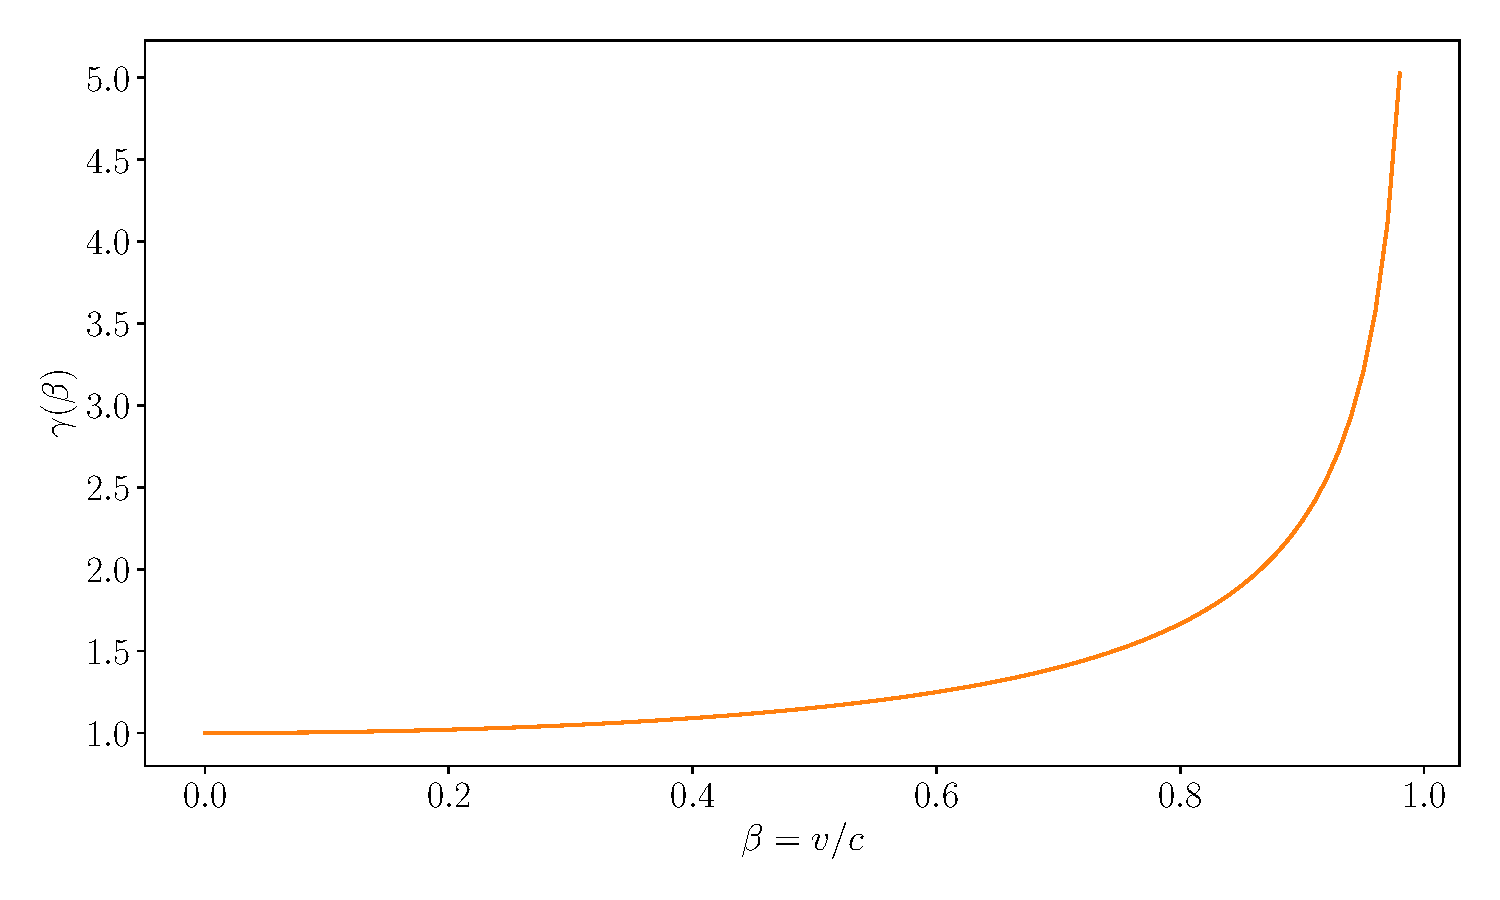
\includegraphics[width=0.9\textwidth]{gamma_factor.pdf}
	
	\caption[Plot of the Lorentz-factor]{Plot of the Lorentz-factor $\gamma = \frac{1}{\sqrt{1 - v^2 / c^2}}$.	Clearly, its effect only becomes significant for speeds which are significant fractions of $c$.}
	\label{fig:gamma_factor}
\end{figure}



\begin{figure}
	\centering

%	\begin{minipage}{0.5\textwidth}
%		\centering

		\begin{tikzpicture}
			\spacetimediagram[onlypositive=true, lightcone=false]{4}
	
			\draw[thick, red, cm={1, 0, 1/2, 1, (0,0)}] (0, 0) rectangle (2, 4);  % "World line" of rod
			\draw[thick, red, dashed, cm={1, 0, 1/2, 1, (0,0)}] (1, 0) -- (1, 4);  % World line of midpoint -> yes, for condition of simultaneity
	
			\draw[thick, lightyellow] (0, 0) -- (2, 2);
			\draw[thick, lightyellow] (0, 4) -- (8/3, 4/3);
	
			\draw[->, thick, blue] (0, 0) -- (4, 2) node[right] {$x'$};
			\draw[->, thick, blue] (2, 4) -- (2.5, 5) node[above] {$ct'$};
	
		\end{tikzpicture}
%	\end{minipage}%
	%
%	\begin{minipage}{0.5\textwidth}
		%\centering

		\caption[Spacetime diagram for a moving rod]{Spacetime diagram for a rod moving with velocity $v$, whose ends are depicted as red lines (midpoint using dashed line).\\
		By definition, the axis $ct'$ is the left end of the rod at $x' = 0$. In the $(ct, x)$-frame, it is given by the line $x = vt$. For the $x'$-axis, one can construct the point on the world line of the right end of the rod that is simultaneous to $t' = 0$ as measured by the left end of the rod. In accordance with the Einstein synchronization, this can be done by looking at light sent out from the origin and its intersection with the midpoint (dashed line). Tracing back this intersection point using light that is sent out by the right end of the rod in negative $x$-direction, one finds the point simultaneous to $t = 0 = t'$ in the origin (i.e.~the line of simultaneity, which is nothing but $x'$).}
		\label{fig:moving_rod_diagram}
%	\end{minipage}
\end{figure}





\iffalse
{ % To complicated
To obtain the way $t \rightarrow t'$ transforms, we have to think a bit more and in fact, reinterpret the ansatz \eqref{eq:lorentz_spatial_ansatz}. 
-> this is the same as arguing in terms of equilocality for moving measuring rod; if we do this for time, i.e.~think about simultaneity, we end up with ...

Demanding the same structure for $t' \rightarrow t$ means


from that we get $\gamma$


\begin{figure}
	\centering
	
	\begin{tikzpicture}
		\spacetimediagram[onlypositive=true, lightcone=false]{4}

		\draw[thick, red, cm={1, 0, 1/2, 1, (0,0)}] (0, 0) rectangle (2, 4);  % "World line" of rod
		\draw[thick, red, dashed, cm={1, 0, 1/2, 1, (0,0)}] (1, 0) -- (1, 4);  % World line of midpoint -> yes, for condition of simultaneity

		\draw[thick, lightyellow] (0, 0) -- (2, 2);
		\draw[thick, lightyellow] (0, 4) -- (8/3, 4/3);

		\draw[->, thick, blue] (0, 0) -- (4, 2) node[right] {$x'$};
		\draw[->, thick, blue] (2, 4) -- (2.5, 5) node[above] {$ct'$};

	\end{tikzpicture}
	
	\caption{}
\end{figure}


In $x$-coordinates, the point $x' = 0$ moves away at speed $x = vt$


the axis $x'$ is determined from the fact that it consists of all events happening at $t' = 0$, i.e.~those which are simultaneous to origin $(ct', x') = (0, 0)$; we have determined this axis by constructing event $E$ that right end of rod perceives to be simultaneous to $t' = 0$ measured by left end of rod (which crosses origin)

rod does not move in primed coordinates, i.e.~$x' = const$ for it; therefore, by prolonging world line of left end of rod, we get axis where $x' = 0$ for all times $t'$ and thus the axis $ct'$


$\gamma$ is stretching, needed because we know that lengths are measured differently in moving systems

}
\fi



		\subsection{Time Dilation \& Length Contraction 2}\label{subsec:time_dilation_lorentz}
In principle, it is not surprising that a new transformation has to be used. After all, we have demanded some new postulates to be true and there is no reason for the \enquote{old} transformation to fulfil it. On the other hand, we have already examined quite a few predictions of these postulates in the clock section \ref{sec:clocks} and likewise, it is not guaranteed that our new Lorentz transformation reproduces the results which have been found there.

Most prominently, time dilation and length contraction showed up as new effects. We will now check if they can be reproduced in coordinates related via the Lorentz transformation.



			\paragraph{Measuring in Unprimed Coordinates}
Consider a rod with ends at positions $x_1, x_2$. Their spatial distance and thus the length of the rod in unprimed coordinates is
\begin{equation*}
	L = x_2 - x_1 \, .
\end{equation*}

From the primed coordinates, however, one would measure
\begin{equation*}
	L' = x'_2 - x'_1 = \gamma (x_2 - v t_2) - \gamma (x_1 - v t_1) = \gamma (x_2 - x_1) = \gamma L = \frac{L}{\sqrt{1 - \frac{v^2}{x^2}}} \, .
\end{equation*}
Here we assume $t_1 = t_2$ because by definition, distances are measured at the same time (simultaneously). This result is not what we expect from the previous discussions. Is the Lorentz transformation at fault? Luckily, no. We have emphasized how simultaneity is important for the length to be meaningful. However,
\begin{equation}\label{eq:not_simultaneous}
	t'_1 = \gamma (t_1 - \frac{v}{c^2} x_1) \neq \gamma (t_2 - \frac{v}{c^2} x_2) = t'_2
	\quad \Leftrightarrow \quad
	\Delta t' = t'_2 - t'_1 = \gamma \frac{v}{c^2} (x_1 - x_2)
	\, ,
\end{equation}
the measurements in primed coordinates are not simultaneous, so this $L'$ is \emph{not} what a ruler in primed coordinates measures. In order to simulate this result, we have to tune the times $t_1, t_2$ to achieve $t'_1 = t'_2$. Choosing
\begin{equation}
	\Delta t = t_2 - t_1 = - \Delta t' = - \gamma \frac{v}{c^2} (x_1 - x_2) = \frac{v}{c^2} \gamma L
\end{equation}
leads to a cancellation of the time difference in \eqref{eq:not_simultaneous}. The \enquote{true} length measured in unprimed coordinates then becomes
\begin{equation}
	\begin{split}
	\eqbox{L'} &= x'_2 - x'_1 = \gamma (x_2 - v t_2) - \gamma (x_1 - v t_1) = \gamma L - v \Delta t
	\\
	&= \gamma L - \frac{v^2}{c^2} \gamma L = \frac{1 - \frac{v^2}{c^2}}{\sqrt{1 - \frac{v^2}{c^2}}} L = \sqrt{1 - \frac{v^2}{c^2}} L = \eqbox{\frac{L}{\gamma}} \, .
	\end{split}
\end{equation}
Moving rulers measure smaller distances, physics is still intact.
Effectively, this corresponds to waiting a longer time until the second measurement in unprimed coordinates, which in turn causes the transformed times $t'_1, t'_2$ to be equal (note that the length $L$ does not change because it is at rest in unprimed coordinates, i.e.~$x_1, x_2$ are constant, independent of time). An intuitive explanation for this is that the moving observer claims the system at rest is moving, i.e.~the end of the rod moves away from him, shortening it. In order to compensate for that, we have to wait a bit longer until taking the second measurement at $t'_2$ and correspondingly, increase $t_2$.\\


Consider a temporal distances $T = t_2 - t_1$ measured by a clock resting in unprimed coordinates (i.e.~$x_1 = x_2$). This time difference measured from primed coordinates is
\begin{equation*}
	%T = t_2 - t_1
	%\qquad \qquad
	T' = t'_2 - t'_1 = \gamma (t_2 - \frac{v}{c^2} x_2) - \gamma (t_1 - \frac{v}{c^2} x_1) = \gamma (t_2 - t_1) = \gamma T = \frac{T}{\sqrt{1 - \frac{v^2}{c^2}}} \, .
\end{equation*}
The primed observer measures a time $T'$ between two events on his clock, while on the clock resting in unprimed coordinates,
\begin{equation}
	\eqbox{
	T = \sqrt{1 - v^2 / c^2} \, T'
	}
\end{equation}
go by. Since the primed observer sees the unprimed one moving, that confirms what we already knew: moving clocks tick slower. This effect can be attributed to the synchronization of clocks. Despite $x_1 = x_2$, $x'_1 \neq x'_2$, so the measurements in primed coordinates are taken by two different clocks (which are properly synchronized, but in the primed frame).



			\paragraph{Measuring in Primed Coordinates}
Now consider a rod with end points at $x'_1, x'_2$. Its length measured in primed coordinates is
\begin{equation*}\label{eq:rod_primed_coords_from_primed}
	L' = x'_2 - x'_1 \, .
\end{equation*}

This measurement is conducted simultaneously in primed coordinates, so $t'_1 = t'_2$. From unprimed coordinates, however, we measure at $t_1 = t_2$. For this reason, $L'$ becomes
\begin{equation*}
	L' = x'_2 - x'_1 = \gamma (x_2 - v t_2) - \gamma (x_1 - v t_1) = \gamma (x_2 - x_1) = \gamma L \, .
\end{equation*}
Consequently, the length $L$ of the rod measured in unprimed coordinates is
\begin{equation}
	\eqbox{
	L = \frac{L'}{\gamma}
	} \, ,
\end{equation}
which confirms the mutuality of length contraction.


Next, consider a temporal distance $T' = t'_2 - t'_1$ measured by a clock resting in primed coordinates (i.e.~$x'_1 = x'_2$). Measuring in this difference in unprimed coordinates, where the clock has moved from $x_1$ to $x_2 = x_1 + v T, \; T = t_2 - t_1$ during this time, yields
\begin{equation}
	\eqbox{T'} = t'_2 - t'_1 = \gamma (t_2 - \frac{v}{c^2} x_2) - \gamma (t_1 - \frac{v}{c^2} x_1) = \gamma (t_2 - t_1 - \frac{v^2}{c^2} T) \eqbox{= \frac{T}{\gamma}} \, .
\end{equation}
Hence, we have also obtained the mutuality of time dilation.\\


Albeit the calculations are largely equivalent, we have argued slightly differently here, which was done deliberately to show there is not a single correct way of calculating the corresponding effects. In the end, we can can confirm that both length contraction and time dilation are reproduced by the Lorentz transformation. Furthermore, the calculations are much more straightforward compared to what had to be done previously (setting up synchronization, drawing complicated diagrams etc.). For this reason, it is customary to introduce the Lorentz transformation without covering any details on clocks. However, in my personal experience, that often results in a lack of intuition on these topics -- one is bound to the understanding in terms of Lorentz transformations, although they are \emph{not} necessary to understand what is going on. Since special relativity is a confusing topic in itself due to several frames and new concepts, intuition is an important part and helps tremendously with interpreting calculations.



		\subsection{Addition of Velocities}

follow Giulini 2.4?


result for relativistic addition $+_R$ (for parallel velocities):
\begin{equation}\label{eq:velocity_addition_parallel}
	\eqbox{
	v +_R w = \frac{v + w}{1 + v w / c^2}
	}
\end{equation}



		\subsection{Spacetime Diagrams 2}
Even more help with understanding relativity is provided by visualizations like spacetime diagrams, which are especially helpful because one can visualize multiple observers in a single diagram (see e.g.~fig.~\ref{fig:moving_rod_diagram} or fig.~\ref{fig:spacetime_diagram_two_observers}, where grid lines are shown as well). Essentially, this is a geometric way of visualizing what Lorentz transformations do. By marking the coordinates $(x, ct)$ of an event in a single, resting frame we can immediately read off the coordinates in other frames as well by showing the axes as it is done in \ref{fig:spacetime_diagram_two_observers}. In principle, a Lorentz transformation shifts the points $(x, ct) = (0, ct)$ by $-vt$ to the left. This means the $ct'$-axis is rotated to the left compared to the $ct$-axis, so events would have different positions in diagrams. For this reason, the $ct'$-axis is rotated to the right, such that the position of events stays the same (an analogous argument can be made for the $x'$-axis). Reading off coordinates then works by looking at the transformed lines of simultaneity (parallel to $x'$-axis) and equilocality (parallel to $ct'$-axis), i.e.~projecting the event parallel to these lines until we find the intersection with the $ct'$- and $x$-axis, respectively.


%explanation why primed axes are shifted inwards in Minkowski diagrams: we wish to express these axes in the unprimed coordinate system, i.e.~we do not apply the Lorentz transform from unprimed (at rest) to primed (moving with $v$), but rather the inverse one (thus we have to use $-v$ in transformation) -> better explanation: we wish to draw only one point for events; since a coordinate change from unprimed to primed would rotate the $ct$-axis (where $x = 0$) by $-vt$ and thus to the left ($ct'$ would then by $y$-axis), we have to rotate the $ct'$-axis by the same amount to the right; then, we can read off coordinates of an event in the unprimed and primed frame at once


We have already discussed the causal structure of relativity, timelike trajectories are always in the light cone and spacelike ones are outside of it. For this reason, the events marked by red dots in figure \ref{fig:spacetime_diagram_spacelike} are clearly spacelike. Now we get a a visual explanation of why spacelike events are problematic: while the unprimed, resting observer sees the left event $E_1$ happening before the right one $E_2$, the primed observer sees $E_2$ happening before $E_1$. Thus, if $c$ was not the speed limit and spacelike events were able to communicate with each other, observers could disagree on cause and effect. Luckily, no evidence for such a transmission with $v > c$ has been found (yet), so we do not have to rebuild our understanding of causality.\\



\begin{figure}
	\centering
	
	\begin{tikzpicture}[scale=1.2]
		% Declare numbers as tikz variables, makes changing very convenient
		\tikzmath{\v = 0.5;}

		% Add basis for diagram
		\spacetimediagram{4}
	
		% Add other observer (one sufficient, for more diagram gets increasingly confusing)
		\addobserver{3}{\v}
	
		%\lightcone{1}{-1}{1}{2}
	
		% Add event in rest frame
		\addevent{0}{2}
		\addevent{2}{2}
	
		% Add same event in moving frame
		\addevent[v=\v, color=blue]{0}{2}
		\addevent[v=\v, color=blue]{2}{2}
	\end{tikzpicture}
	
	\caption[Events in frames moving with $v = 0.5 c$ relative to each other]{Events in frames moving with $v = 0.5 c$ relative to each other. Red dots show two events at spacetime points $(x, ct) = (0,2), (2,2)$ (the corresponding primed coordinates are $(x', ct') = (-1.15, 2.3), (1.15, 1.15)$). Blue dots show the same coordinates in the $(x', ct')$-frame (corresponding unprimed coordinates: $(x, ct) = (1.15, 2.3), (3.46, 3.46)$).\\
	We can see very nicely how each observer perceives time differently. Events happening simultaneously to both red dots (i.e.~which lie on the line between them at $t = 2$), do \emph{not} happen at $t' = t$, but at $t' = \tau = \sqrt{1 - v^2} \, t$ (which is evident from the fact that the blue dots are at $t' = t$). The same can be said for the moving observer in blue, which sees events at $t = \sqrt{1 - v^2} \, t'$ simultaneous to the blue dots at $t' = 2$. Analogous arguments can be made for positions and equilocality.}
	\label{fig:spacetime_diagram_two_observers}
\end{figure}



\begin{figure}
	\centering
	
	\begin{tikzpicture}[scale=1.2]
		% Declare numbers as tikz variables, makes changing very convenient
		\tikzmath{\v = 0.5;
				  \Eonex = -1; \Eoney = 2;
				  \Etwox = 2.5; \Etwoy = 3; % For spacelike, velocity times x-coordinate difference has to be greater than time-coordinate difference
				 }

		% Add basis for diagram
		\spacetimediagram[lightcone=false]{4}
	
		% Add other observer (one sufficient, for more diagram gets increasingly confusing)
		\addobserver{3}{\v}
	
	
		% Add event in rest frame
		\lightcone[xpos=\Eonex, ypos=\Eoney]{2}
		\addevent[label=$E_1$]{\Eonex}{\Eoney}
		\addevent[label=$E_2$]{\Etwox}{\Etwoy}
	\end{tikzpicture}
	
	\caption[Spacelike events]{Spacelike events.\\
	It is very obvious that $E_2$ does not lie in the light cone of $E_1$, which has been visualized to make that clear (this implies $E_1$ does not lie in the light cone of $E_2$). The unprimed, black observer sees $E_1$ happening before $E_2$, while the blue observer moving at $v = 0.5 c$ sees it the other way around.}
	\label{fig:spacetime_diagram_spacelike}
\end{figure}



The new addition of being able to depict multiple observers to spacetime diagrams makes them a powerful tool suitable to explain many effects of relativity. For example, the fairly complicated twin paradox can be explained and -- perhaps, even more important -- visualized conveniently.

\begin{ex}[Twin Paradox 2]\label{ex:twin_paradox_2}
	As promised, here comes the detailed demonstration of the twin paradox, which has been started in example \ref{ex:twin_paradox_1}. We will discuss the setup shown in figure \ref{fig:twin_paradox}, i.e.~treat one observer at rest (will be commonly referred to as \enquote{unprimed} one) and two observers moving with velocities $v = \pm 0.5 c$ relative to the unprimed observer (these will be called \enquote{primed} and \enquote{double-primed}, in accordance with their axis labels in \ref{fig:twin_paradox}).
	
	Our approach will be to compute the roundtrip time needed to go from $S$ to $E$ (i.e.~the time passing on the world line on $ct$ axis) and the time needed to go from $S$ to $T$ to $E$ (i.e.~the time passing on the other world line shown in \ref{fig:twin_paradox}). Each of these quantities will be computed from clocks resting in all three of the inertial frames shown in figure \ref{fig:twin_paradox} (reminder: three are involved due to turning around, rest frame of moving observer changes there).
	
	%the thing that makes things make sense is that all observers agree on the time passing along moving clock, even when measured from their coordinates; after all, from the double-primed coordinates we can still look at time passing on clock in primed coordinates and simultaneously passing in rest frame; adding that up, we get the total times and these agree between the frames (good, otherwise we would have problem)
	
	During the process, we have to distinguish between four times: (i) the time $t_{ST}$ passing on the resting clock between $S$ and $T$, (ii) the time $t_{TE}$ passing on the resting clock between $T$ and $E$, (iii) the time $\tau_{ST}$ passing on the moving clock between $S$ and $T$ and (iv) the time $\tau_{TE}$ passing on the moving clock between $T$ and $E$. From that we get the total times for resting and moving clock,
	\begin{equation*}
		t_{SE} = t_{ST} + t_{TE}
		\manyqquad
		\tau_{SE} = \tau_{ST} + \tau_{TE} = t'_{ST} + t''_{TE} \, .
	\end{equation*}
	
	One final note concerns the velocities involved: the world line is drawn for $v = 0.5 c$ on the way from $S$ to $T$ and $v = -0.5 c$ on the way from $T$ to $E$ (same velocity, different direction), where $v$ is the velocity of the respective moving frame compared to the unprimed, resting one. This implies a relative velocity of $v_2 = \frac{0.5 c + 0.5 c}{1 + 0.5^2} = 0.8 c$ from double-primed to primed frame (note that addition of velocities works differently in relativity).
	
	\begin{itemize}
		\item \textbf{Measuring from unprimed coordinates}
		
		Clearly,
		\begin{equation*}
			t_{ST} = 2 = t_{TE}
			\qquad \Leftrightarrow \qquad
			t_{SE} = t_{ST} + t_{TE} = 4
		\end{equation*}
		in arbitrary time units (where one time unit goes by between two grid lines). From that, Minkowski's theorem tells us
		\begin{equation*}
			t'_{SE} = \sqrt{1 - v^2} \, t_{SE} = 3.464 \, .
		\end{equation*}
	
		Simultaneously, by looking at how much time elapses between the intersection of gray grid lines and the blue $ct'$-axis, one can see that as a rough estimate $t'_{ST} \lesssim 2$. For the exact result, we apply Minkowski's theorem:
		\begin{equation*}
			t'_{ST} = \tau_{ST} = \sqrt{1 - v^2 / c^2} \, t_{ST} = \sqrt{1 - 0.5^2} \cdot 2 = 1.732 \, .
		\end{equation*}
		Applying the same procedure to the double-primed coordinates yields
		\begin{equation*}
			t''_{TE} = \tau_{TE} = \sqrt{1 - v^2 / c^2} \, t_{TE} = \sqrt{1 - (-0.5)^2} \cdot 2 = 1.732 = \tau_{ST} \, .
		\end{equation*}
		
		This is because time dilation does not depend on the direction, only on the absolute velocity. Therefore, we can confirm that
		\begin{equation*}
			t_{SE} = t_{ST} + t_{TE} = 4 > \tau_{SE} = \tau_{ST} + \tau_{TE} = 3.464 \, ,
		\end{equation*}
		less time goes by on the moving clock.
		
	
	
		\item \textbf{Measuring from primed coordinates}
	
		While from these coordinates one still sees four time units going by on the roundtrip for the resting observer, i.e.~$t_{SE} = 4$, a rough estimate for the roundtrip time measured by a clock resting in the primed coordinates $ct'$ is $t'_{SE} \gtrsim 4$. More precisely, Minkowski's theorem yields
		\begin{equation*}
			t_{SE} = \sqrt{1 - v^2 / c^2} \, t'_{SE}
			\qquad \Leftrightarrow \qquad
			t'_{SE} = \frac{t_{SE}}{\sqrt{1 - v^2 / c^2}} = \frac{4}{\sqrt{1 - (-0.5)^2}} = 4.619 \, .
		\end{equation*}
		This is a consequence from the mutuality of time dilation, an observer resting in primed coordinates sees the unprimed observer moving at $v = -0.5 c$ and therefore measures more time passing in his own frame.
	
	
		However, $t'_{SE}$ is not what a clock in the primed coordinates sees. Instead, 
		\begin{equation*}
			\tau_{SE} = \tau_{ST} + \tau_{TE} = t'_{ST} + t''_{TE}
		\end{equation*}
		as stated before. For $t'_{ST}$, however, we cannot simply use Minkowski's theorem and thus the time
		\begin{equation*}
			\frac{t_{ST}}{\sqrt{1 - v^2 / c^2}} = 2.309 \, ,
		\end{equation*}
		which cannot be quite correct since from the diagram we get the estimate $t'_{ST} \lesssim 3$. This is because the world line is moving with respect to the rest frame of $ct$, so we would only get statements about what is the time as seen from this frame. However, we wish to measure the primed time from the primed coordinates. This requires a Lorentz transformation of the events $S, T, E$:
		\begin{equation*}
			t'_{ST} = t'_T - t'_S = \frac{t_T - \frac{v}{c} x_T}{\sqrt{1 - v^2 / c^2}} - \frac{t_S - \frac{v}{c} x_S}{\sqrt{1 - v^2 / c^2}} = \frac{t_{ST} - \frac{v}{c} x_T}{\sqrt{1 - v^2 / c^2}} = \frac{2 - 0.5 \cdot 1}{\sqrt{1 - 0.5^2}} = 1.732 \, .
		\end{equation*}
		In the same manner, we obtain
		\begin{equation*}
			t'_{TE} = t'_E - t'_T = \frac{t_E - \frac{v}{c} x_E}{\sqrt{1 - v^2 / c^2}} - \frac{t_T - \frac{v}{c} x_T}{\sqrt{1 - v^2 / c^2}} = \frac{t_{TE} + \frac{v}{c} x_T}{\sqrt{1 - v^2 / c^2}} = \frac{2 + 0.5 \cdot 1}{\sqrt{1 - (-0.5)^2}} = 2.887 \, .
		\end{equation*}
	
		To get $t''_{TE}$, we have to prolong the axes of simultaneity of the primed coordinates and count the number of time units which go by between the intersections of them with $ct''$ (i.e.~the number of intersections with green lines on the way). This yields roughly $t''_{TE} \gtrsim 1.5$ again. For the time passing simultaneously on a clock in primed coordinates, we can read off roughly $t'_{TE} \approx 4$. The correct numbers can be obtained from Minkowski's theorem again:
		\begin{equation*}
			t''_{TE} = \sqrt{1 - (-v_2)^2 / c^2} \, t'_{TE} = \sqrt{1 - (-0.8)^2} \, 2.887 = 1.732 \, .
		\end{equation*}
	
		All together, the primed observer measures a roundtrip time
		\begin{equation*}
			t'_{SE} = t'_{ST} + t'_{TE} = 4.619 > \tau_{SE} = \tau_{ST} + \tau_{TE} = t'_{ST} + t''_{TE} = 3.464 \, .
		\end{equation*}
		We find the same result that less time has passed on the moving clock. Furthermore, we see that the absolute value for this $\tau_{SE} = t'_{SE}$ and the one computed from Minkowski's theorem in the first calculation agree (because corresponding world line is parallel to $ct$, i.e.~in rest frame). On the other hand, it should not be surprising that the absolute values measured for $\tau_{ST}$ and $\tau_{TE}$ do not agree. After all, they are still measured from different inertial frames and they measure with respect to frames moving with different relative velocities ($\pm 0.5$ for primed; $0.5, 0.8$ for unprimed).
	
		
		% for v=0.7 c
		%on own clock, six time units go by for roundtrip; however, he agrees that just four go by on resting clock
		
		%on own clock, it is again roughly $3 / 2$ which pass by; on $ct''$ he sees $3 / 2$ passing by as well (way to see that: look at which lines parallel to $x'$ intersect the relevant events, i.e.~starting point and turning point; then look at points where these lines intersect $ct''$ and count number of ticks on $ct''$ between these intersections); in the same manner, we see that four time units pass on $ct$
		
		\item \textbf{Measuring from double-primed coordinates}
	
		Just as before, $t_{SE} = 4$ is measured, while roughly $t''_{SE} \gtrsim 4$ and precisely
		\begin{equation*}
			t''_{SE} = \frac{t_{SE}}{\sqrt{1 - v^2 / c^2}} = \frac{4}{\sqrt{1 - (-0.5)^2}} = 4.619
		\end{equation*}
		are measured by a clock resting in the double-primed coordinates. As one can confirm by looking at the result above, this is the same time a clock resting in primed coordinates measures. We expect more of these equal results since the double-primed coordinate system is moves with the same relative velocity as the primed one, just in the other direction (sign of velocity is different).
	
		A rough estimate for $t''_{TE}$ is $t''_{TE} \gtrsim 2$ and the exact result is
		\begin{equation*}
			t''_{TE} = t''_E - t''_T = \frac{t_E - \frac{v}{c} x_E}{\sqrt{1 - v^2 / c^2}} - \frac{t_T - \frac{v}{c} x_T}{\sqrt{1 - v^2 / c^2}} = \frac{t_{TE} + \frac{v}{c} x_T}{\sqrt{1 - v^2 / c^2}} = \frac{2 - 0.5 \cdot 1}{\sqrt{1 - (-0.5)^2}} = 1.732 \, .
		\end{equation*}
		An analogous calculation yields
		\begin{equation*}
			t''_{ST} = t''_T - t''_S = \frac{t_T - \frac{v}{c} x_T}{\sqrt{1 - v^2 / c^2}} - \frac{t_S - \frac{v}{c} x_S}{\sqrt{1 - v^2 / c^2}} = \frac{t_{ST} - \frac{v}{c} x_T}{\sqrt{1 - v^2 / c^2}} = \frac{2 + 0.5 \cdot 1}{\sqrt{1 - 0.5^2}} = 2.887 \, .
		\end{equation*}
		As promised, we get more results that we have already seen when making computations in the primed coordinates, but now they are switched (due to the transition $v \rightarrow -v$).
	
		Now we wish to compute $t'_{ST}$ and expect the rough estimate $t'_{ST} \gtrsim 1.5$. Indeed, we obtain
		\begin{equation*}
			t'_{ST} = \sqrt{1 - v_2^2 / c^2} \, t'_{TE} = \sqrt{1 - 0.8^2} \, 2.887 = 1.732 \, .
		\end{equation*}
		All in all, the double-primed observer measures a roundtrip time
		\begin{equation*}
			t''_{SE} = t''_{ST} + t''_{TE} = 4.619 > \tau_{SE} = \tau_{ST} + \tau_{TE} = t'_{ST} + t''_{TE} = 3.464 \, .
		\end{equation*}
		Once again, these results look very familiar. 
	\end{itemize}
	
	A conclusion of these extensive calculations is that physics is not broken, despite relativity sometimes being unintuitive at first glance. Although all inertial frames play equal roles, which shows in the mutual slowing of moving clocks, all agree on the effect of time dilation: moving clocks tick slower than resting ones. In frames where both clocks seem to be moving, we can further confirm that the effect increases with the velocity $v$.
	
	It should also be noted that the agreement of all three observers regarding $\tau_{SE}$ is really a coincidence due to the symmetric setup we have chosen -- for other scenarios, e.g.~with unequal velocities on the first and second part of the journey or perhaps even if we assume that $ct$ is not at rest after all (but keeping the relative velocities of primed and unprimed system, i.e.~rotating the whole setup), this will not be the case anymore. In the same manner, $t'_{ST} \neq t''_{TE}$ in general. However, if one of the clocks moves on a world line parallel to the $ct$-axis of one of the observers, \emph{all} of them will agree on the time elapsed along this clock (so $t_{SE}$ being equal for all observers is really not a coincidence; the same goes for $t'_{ST}$ and $t''_{TE}$ in this setup). This is despite observers measuring different times on their own clocks and is due to Minkowski's theorem, which tells us how much time has passed simultaneously on a clock in another frame.


-> note: although there is no preferred system in the sense that it is \enquote{more correct} than others (no absolute space), one can argue it numbers computed in stationary system are the ones that make most sense because assuming the moving observer stops again and rests after his journey, this rest frame is where they compare their clocks in and thus also where an experiment would be conducted (i.e.~these times would be the one which are measured)
\end{ex}



\begin{figure}
	\centering

	\begin{tikzpicture}[scale=1.2]
		% Declare numbers as tikz variables, makes changing very convenient
		\tikzmath{\vprime = 0.5; \vdoubleprime = -0.5;
				  \tS = -2; \tT = 0;
				  \tE = 2; \xS = 0;
				  \xT = (\tT - \tS) * \vprime; \xE = 0;
				  }  % Note: world line connecting S and T is always parallel to time axis of primed observer, while world line connecting T and E is only parallel to double-primed if vprime=-vdoubleprime

		% Add basis for diagram
		\spacetimediagram{4}
	
		% Add other observers
		\addobserver{3}{\vprime}
		\addobserver[xlabel=$x''$, ylabel=$ct''$, color=black!40!green]{3}{\vdoubleprime}

		% Add worldlines of clocks and start, end events
		\addworldline{\xS}{\tS}{\xT}{\tT}  % Resting clock
		\addworldline{\xS}{\tS}{\xT}{\tT}  % Moving clock
		\addworldline{\xT}{\tT}{\xE}{\tE}  % Moving clock

		\addevent[radius=2pt, label=$S$, label placement=right]{\xS}{\tS}  % S
		\addevent[radius=2pt, label=$T$, label placement=right]{\xT}{\tT}  % T
		\addevent[radius=2pt, label=$E$, label placement=right]{\xE}{\tE}  % E
	\end{tikzpicture}

	\caption[Visual explanation of twin paradox]{Visual explanation of twin paradox. Event $S$ is the starting point, $T$ turning point and $E$ end point. The primed observer has a relative velocity of $v = 0.5 v$ with respect to the unprimed one, while the double-primed observer has $v = -0.5 c$.\\
	We can measure times passing between events in a certain frame $\mathcal{O}$ by prolonging the corresponding lines of simultaneity (parallel to spatial axis of $\mathcal{O}$) from event to the time axis of $\mathcal{O}$ and then count the number of time units passing on the time axis between the intersection points. Similarly, we could also prolong them until they intersect the time axis of any other frame $\mathcal{O}'$. In this case, counting the number of time steps passing between the intersection points on the time axis of $\mathcal{O}'$ would yield the time passing for $\mathcal{O}'$, measured from $\mathcal{O}$.}
	\label{fig:twin_paradox}
\end{figure}



\newpage



	\section{Minkowski Space}
Throughout the last sections, we discovered more and more how space and time work in relativity and how they are related. Important contributions to that picture were made by the insights of Einstein regarding synchronization of clocks and Lorentz, who developed a corrected version of the Galilei transform.

It might be clear to the reader that this implies space and time are not independent anymore, but instead have to be treated on the same footing. Historically speaking, however, this final step was not made until Minkowski proposed his viewpoint that physics should take place in a four-dimensional \Def{spacetime}. This unification is an essential part of how the theory of relativity is described in modern literature, in particular because it allows a description in terms of a well-developed mathematical theory -- the theory of manifolds. We will also adopt the usage from now on.


% over the course of the last sections, we saw more and more how space time work in relativity and how they are related; Einstein's insights and Lorentz transform show how clocks work differently than their Newtonian pendants once relativity principle is incorporated, they are not independent anymore; but it is only with the Minkowskian viewpoint that this connection is fully unveiled/completed by uniting them into one spacetime (which goes along with unified mathematical formulation on sound/fond footing)


% ok, this might be nice: in spacetime diagrams, we see the idea how space and time (which are, as we know now, no separate notions) can be combined into one entity -- describe them as coordinates in one space; this space is called Minkowski space and spacetime diagrams can be seen as a visualization of it; SR is basically which geometry Minkowski space possesses and mathematically, we can describe that in metric; this metric we get from invariant notion we have already seen




%		\subsection{Basic Definitions}
First, it is necessary to state what spacetime is in a formal, mathematical way.


\begin{defi}[Minkowski Space]
	In special relativity, \Def{Spacetime} is described as a $4$-manifold $M$ with one time and three spatial coordinates. Another common name for $M$ is \Def{Minkowski space} with corresponding symbol $\mathbb{M}$ (i.e.~we use $M = \mathbb{M}$).

	\Def{Events} $E$ are points in $M$ and they can be specified using \Def{inertial Cartesian coordinates} as
	\begin{equation}
		\eqbox{
		\underline{x} = (ct, x, y, z) = (ct, \vec{x})
		}
	\end{equation}
	where $(x, y, z)$ are the Cartesian coordinates of Euclidian space.
	
	
	\Def{World lines} are curves $\Gamma = \Gamma(\sigma): I = [a, b] \rightarrow M$.
\end{defi}
We adopt the convention to rescale the time-component to have the same units as the spatial components. To avoid these conversion factors, we could choose units where $c = 1$, as it is common practice when dealing with relativity. However, we have elected not to do this here. Another note on the coordinates is that choosing inertial Cartesian coordinates is by no means necessary, just like spherical coordinates are equally suited to describe physics in Euclidian space as Cartesian ones. It is simply more convenient for now and we maintain generality of our discussion because the theory of manifolds provides us with natural ways of changing coordinates. This mathematical way of demanding coordinate-independent statements and using invariant notions like tensors is completely equivalent to what relativity demanded: physics has to be invariant of the observer, so only special quantities like proper times have an invariant and thus physical meaning (coordinate times or positions do not). This correspondence of underlying ideas and concepts is the reason why describing relativity in the language of manifolds is a very natural idea.


Having defined spacetime, we can see why space-time diagrams have been called spacetime diagrams: they visualize the new-defined entity $M$, just like coordinate planes with $x$-, $y$-axis visualize Euclidian space. This also explains why they are often called \Def{Minkowski diagrams}.\\


While points and vectors do not necessarily have a direct identification with each other, elements of the vector space $\mathbb{M}$ are also points in $M$ because both are elements of $\mathbb{R}^4$ (which further motivates $M = \mathbb{R}^4$).\footnote{To be more precise, $\mathbb{M}$ is the affine space of $\mathbb{R}^4$, i.e.~we keep the space itself, but not the attached notions of distances and angles. In particular, there is no origin (in accordance with relativity principle).} For this reason, $\underline{x} = (ct, x, y, z)$ is often called four-vector. Over the course of the next sections, we will develop the mathematical tools to describe spacetime. As we will learn throughout this section, it has more structure than what is natively given by \enquote{pure} manifolds, namely a metric. Therefore, $\mathbb{M}$ will turn out to be a \Def{pseudo-Riemannian manifold} or \Def{Lorentz-manifold}, $\mathbb{M} = (\mathbb{R}^4, \eta)$. At this point, the departure from Euclidian space with metric $g$ and line element $ds^2 = dt^2 + dx^2 + dy^2 + dz^2$ begins.


%introduce four-velocity as tangent vector; then also state that as of now, we are not able to take norm of it -> motivates metric section




		\subsection{Metric \& Inner Product}
We have now seen how physics can be conveniently described using a 4D manifold, which we called spacetime. Points on this manifold are events and we can change coordinates or inertial frames using Lorentz-transformations. Moreover, there are several quantities that can be defined naturally on manifolds, for example curves, vectors, and covectors (maps that take vectors as input). While manifolds do have an additional natural structure, this is given by topology. In physics, however, we are also interested in statements concerned with distances between events and to measure them we need additional structure. More specifically, we have to specify a metric that will allow measuring distances, as well as norms of vectors via the induced inner product.


Mathematically, metrics are objects called tensors and they have the convenient property that they are invariant under coordinate changes. Therefore, distances are physically meaningful statements because they do not depend on the inertial frame we compute them on. In the tradition of invariant quantities that have been encountered so far, we may guess that the metric will be related to light in some way. From the universality of the speed if light $c$, distances $s$ are equivalent to times $t$ for light, $s = c t$. Because of that, a natural measure for distances is the time elapsed on a clock, i.e.~the geometric structure of Minkowski space is determined by Minkowski's theorem \ref{thm:minkowski_moving_clocks}. Instead of denoting time with the usual variable $t$, we will now switch to the \Def{proper time} $\tau$ since the time elapsed a clock between events $(0, 0, 0, 0)$ and $(ct, x, y, z)$ is
\begin{equation}\label{eq:proper_time_uniform}
	\eqbox{
	\tau = \sqrt{1 - \frac{v^2}{c^2}} \, t = \sqrt{1 - \qty(\frac{x}{ct})^2 - \qty(\frac{y}{ct})^2 - \qty(\frac{z}{ct})^2} \, t = \sqrt{t^2 - (x^2 + y^2 + z^2) / c^2}
	}
\end{equation}
This distance notion depends on the trajectory taken by the clock/corresponding observer (more specifically, on the uniform velocity $v$), but will in general not be equal to $t$, which is the time measured simultaneously by a clock resting in the corresponding frame. This does \emph{not} mean $\tau$ depends on the coordinates we use to compute it, i.e.~the specific inertial frame chosen, the striking factor is the path taken by the clock we measure time for.



\begin{ex}[Proper Time vs.~Coordinate Time]
	We will use an example to elaborate a bit more on the meaning of all the symbols in \eqref{eq:proper_time_uniform}. Say we are in an inertial frame with coordinates $(ct, x, y, z)$. 
	
	The time elapsed between two events 
	A clock resting in this frame will measure the proper time between events $E_1 = (ct_1, 0, 0, 0), E_2 = (ct_2, 0, 0, 0)$, i.e.~it will show
	\begin{equation*}
		\tau_{E_2, E_1} = t_2 - t_1
	\end{equation*}
	to be elapsed between them. If we look at events $E_3 = (ct_1, x_1, y_1, z_1), E_4 = (ct_2, x_2, y_2, z_2)$, however, it will still measure $t_2 - t_1$. This is not equal to the proper time
	\begin{equation*}
		\tau_{E_3, E_4} = \sqrt{(t_2 - t_1)^2 - ((x_2 - x_1)^2 + (y_2 - y_1)^2 + (z_2 - z_1)^2) / c}
	\end{equation*}
	between these events, which would be measured by a clock moving on the straight world line that connects them.
	
	
	
	Going to a frame with coordinates $(ct', x', y', z')$, which moves uniformly between $E_3$ and $E_4$, the situation is different. A clock resting in this frame moves on a trajectory between $E_3$ and $E_4$, which means the time $t'$ measured by it now coincides with the proper time between these two events,
	\begin{equation*}
		\tau_{E_3, E_4} = t'_2 - t'_1 \, .
	\end{equation*}
	This is because the spatial coordinates of $E_3$ and $E_4$ are equal in the primed frame, the Lorentz transformation automatically incorporates all spatial movement happening in unprimed coordinates into $t'$. However,
	\begin{equation*}
		t'_2 - t'_1 = \tau_{E_1, E_2} = \sqrt{(t'_2 - t'_1)^2 - ((x'_2 - x'_1)^2 + (y'_2 - y'_1)^2 + (z'_2 - z'_1)^2) / c}
	\end{equation*}
	because the trajectory connecting $E_1$ and $E_2$ is not parallel to $ct'$. This is the mutuality of time dilation. Nonetheless, it shows a general way how different observers can agree on times: by using the proper time between events. Not only do the numbers agree in this case, conceptually it also makes a lot of sense to look at times which are measured by clocks which actually \enquote{see} both events, i.e.~move on a world line connecting them, instead of using clocks far away from the event.\\
	
	
	This whole behaviour might seem familiar, we have already encountered it in example \ref{ex:twin_paradox_2}, where the twin paradox has been discussed in detail. Here it already showed how different observers do not necessarily agree on times $t$ their own clocks measure between two events, but they do agree on times they infer to be measured by a clock moving on a trajectory connecting these two events -- the proper time. Moreover, since all observers agree on the proper time, one can immediately infer effects like time dilation, which becomes as easy as
	\begin{equation*}
		t'_2 - t'_1 = \tau'_{E_3, E_4} = \tau_{E_3, E_4} < t_2 - t_1 \, ,
	\end{equation*}
	the primed, moving observers measures smaller times than the unprimed, resting one.
\end{ex}

As we have seen in this example, in some coordinates it is very easy to compute proper times because the object or particle we look at is at rest in this frame, which implies that the coordinate time $t$ is already the proper time, $\tau = t$. These coordinates are often given a special name.
\begin{defi}[Instantaneous Rest Frame]
	A frame $(t, x, y, z)$ where
	\begin{equation}
		\eqbox{
		%dx^\mu = 0, \; \forall \mu % dt is not 0
		dx = dy = dz = 0
		\qquad \Rightarrow \qquad d\tau = dt
		}
	\end{equation}
	along the world line of a particle is called \Def{instantaneous rest frame} or \Def{comoving frame}.
\end{defi}
This definition can also be extended to non-uniform velocities $v = v(t)$ because instantaneous rest frames taken at different times are related by Lorentz transforms. We will now see how the general definition of the proper time may be extended to this case.



		\paragraph{Generalized Proper Time}
What was denoted with $\tau$ in equation \eqref{eq:proper_time_uniform}, in reality is a difference $\Delta \tau$ of proper times (just measured with respect to $\tau = 0$), and the same is true for the coordinates $(ct, x, y, z)$. Making these differences infinitesimally small, i.e.~$\Delta \rightarrow d$, we obtain the infinitesimal distance or \Def{proper time element}\footnote{We adopt the common notation $dx^2 := (dx)^2$.}
\begin{equation}
	\eqbox{
	d\tau^2 = dt^2 - \frac{dx^2 + dy^2 + dz^2}{c^2} = (1 - \frac{v^2}{c^2}) \, dt^2 = \gamma^2 \, dt^2
	} \, .
\end{equation}
This implies the following \Def{(proper) line element}
\begin{equation}
	\eqbox{
	ds^2 = c^2 d\tau^2 = c^2 dt^2 - dx^2 - dy^2 - dz^2
	}
\end{equation}
and corresponding \Def{proper distance} $s = c \tau$ between events (note that this implicitly uses the constancy of $c$ again). Writing this line element out in its general form $ds^2 = \eta_{\mu \nu} dx^\mu dx^\nu$ immediately allows to read off the components of the \Def{Minkowski metric} $\eta$, which can be conveniently arranged in a matrix
\begin{equation}\label{eq:minkowski_metric}
	\eqbox{
	\eta = \mqty(1 & 0 & 0 & 0 \\ 0 & -1 & 0 & 0 \\ 0 & 0 & -1 & 0 \\ 0 & 0 & 0 & -1)
	} \, .
\end{equation}
At this point, we shall make a remark regarding the signs: in principle, we could have chosen $\eta$ to have only one minus (in the time component) since only the proper time is constrained by physical observations, while the proper distance could equally well be defined as $ds^2 = - c^2 d\tau^2$. There are good arguments for both conventions, but I personally find it more natural to keep the signs when going from times to distances, which is why signature $(+, -, -, -)$ is adopted here.\\

-> hmmm, maybe choose other convention? Because this reduces to Euclidian metric for simultaneous events, i.e.~$dt = 0$ (at least in the frame where the events are simultaneous); would also make distinction between $ds^2$ and $d\tau^2$ a bit easier...


Perhaps a bit contrary to popular belief (at least that is what many authors claim), the scope special relativity is not restricted to observers with uniform velocities. Using some of the quantities and tools we have just derived, it is possible to extend the description of certain dynamics to observers moving with non-uniform velocities, i.e.~accelerating ones. For distances, this is possible in the scope of integration on manifolds, where the length of a curve $\Gamma(t)$ defined on an interval $I \subset \mathbb{R}$ is
\begin{equation}
	L(\Gamma) = \int_\Gamma ds = \int_I d\Gamma := \int_I \sqrt{g_{\mu \nu} v^\mu v^\nu} \, dt = \int_I \sqrt{g(\underline{v}, \underline{v})} \, dt \, .
\end{equation}
$\underline{v} = \dv{\Gamma(\sigma)}{\sigma}$ is the tangent vector (field) along $\Gamma$. Because we are equipped with a metric $g_{\mu \nu} = \eta_{\mu \nu}$ and corresponding line element $ds = c \, d\tau$, we can compute proper times for arbitrary kinds of movements.
\begin{post}[Clock Postulate]
	Given a world line $\Gamma$ parametrized by $\sigma \in I = [a, b]$, i.e.
	\begin{equation*}
		\Gamma(\sigma): \sigma \mapsto (t, x, y, z) = (t(\sigma), x(\sigma), y(\sigma), z(\sigma)) \, ,
	\end{equation*}
	the proper time elapsed along $\Gamma$ is
	\begin{equation}\label{eq:proper_time_general}
		\eqbox{
		\begin{split}
		\tau &= \int_\Gamma d\tau = \int_\Gamma \gamma(t) \, dt = \int_\Gamma \sqrt{1 - \frac{v(t)^2}{c^2}} \, dt
		\\
		%&= \int_a^b \dv{\tau}{\sigma} \, d\sigma = \int_a^b \sqrt{\qty(\dv{t}{\sigma})^2 - \frac{1}{c^2} \qty(\dv{\vec{x}}{\sigma})^2} \, d\sigma
		&= \int_a^b \dv{\tau}{\sigma} \, d\sigma = \int_a^b \sqrt{\qty(\dv{t}{\sigma})^2 - \frac{1}{c^2} \dv{x^\alpha}{\sigma} \dv{x^\alpha}{\sigma}} \, d\sigma
		\end{split}
		} \, .
	\end{equation}
\end{post}
Note that while this \enquote{derivation} we provided here does make a lot sense, there is no guarantee for it to be correct -- accelerating clocks could be vastly different from uniformly moving and resting ones. For this reason, we call \eqref{eq:proper_time_general} a postulate rather than a property. Once again, experiments have tested this postulate to very high accelerations of $\approx 10^{16} g$ ($g = 9.81 \frac{\metre}{\second^2}$), which showed no dependence on it (only on the speed $v$).

Intuitively, we can see that \eqref{eq:proper_time_general} works because it utilizes infinitesimal steps $d\tau$ where $v(t)$ does not change, so we can apply what we know at this point and integrate up the results from all points (idea is similar to the rectification of curves). It includes the case of uniform movement $v = \text{const.}$, whence the integrand $\gamma$ is constant and evaluation of the integral simply yields $\tau = \gamma (t_b - t_a)$. In case $v = v(t)$, the most convenient formula to use from \eqref{eq:proper_time_general} really depends on what is given -- it may be the parametrization that is explicitly known or the velocity as a function of time.

Instead of $\sigma$, one could also choose arbitrary linear combinations $\sigma' = e \sigma + f$ ($e, f \in \mathbb{R}$) to parametrize $\Gamma$ and then use $d\sigma' = e \, d\sigma$, which means that the integral in \eqref{eq:proper_time_general} is invariant under changes of this \Def{affine parameter}. A very common choice is $\sigma = \tau$ and we will later see how this specific parametrization can be characterized.\\


Another remark on this definition is related to the metric. In coordinates, which are not inertial Cartesian ones, the metric is very likely to have different components $\eta'_{\mu \nu} \neq \eta_{\mu \nu}$. In this case, the last equality would not hold true anymore, although analogous formulas can be obtained from (again, assuming a world line $\Gamma$ with tangent vector $\underline{v}$)
\begin{equation}\label{eq:proper_time_non_cartesian}
	\eqbox{
	%\tau = \int_\Gamma d\tau = \frac{1}{c} \int_I \sqrt{\eta'(\underline{v}, \underline{v})} \, d\sigma = \frac{1}{c} \int_I \sqrt{\eta'_{\mu \nu} dx^\mu(\underline{v}) dx^\nu(\underline{v})} \, d\sigma = \frac{1}{c} \int_I \sqrt{\eta'_{\mu \nu} v^\mu v^\nu} \, d\sigma
	\tau = \int_\Gamma d\tau = \frac{1}{c} \int_I \sqrt{\eta'_{\mu \nu} v^\mu v^\nu} \, d\sigma
	} \, ,
\end{equation}
which still holds due to the transformation rule for integrals. This rule is also what implies the invariance of $\tau$ under the coordinates/frame it is computed in, which is a mathematical way of stating that all observers agree on the proper time.


It is this invariance that allows us to infer statements about the geometry of Minkowski space (where we now assume $v = \text{const.}$ again and thus use \eqref{eq:proper_time_uniform}). In Euclidian space, points of constant distance $s$ lie on a circle around the origin, which is determined by the equation $s^2 = x^2 + y^2 + z^2$. In Minkowski space, events of equal distance lie on a hyperboloid of constant proper times $\tau$ and are determined by
\begin{equation}\label{eq:eichhyperbel}
	\eqbox{
	c^2 \tau^2 = c^2 t^2 - x^2 - y^2 - z^2
	} \, .
\end{equation}
Setting $c \tau = 1$ yields a hyperbola, whose intersection with time axes in spacetime diagrams determines the \enquote{length of one time unit}, a very convenient way to see how moving clocks are perceived to be slower from a resting observers point of view (fig.~\ref{fig:minkowski_with_eichhyperbel}). In the same manner, one can visualize events of equal spatial distance $dx^2 + dy^2 + dz^2$ by looking at
\begin{equation*}
%	x'^2 = \gamma^2 (x - vt)^2
	x^2 + y^2 + z^2 = c^2 t^2 - c^2 \tau^2 = c^2 t^2 - c^2 t'^2 + x'^2 + y'^2 + z'^2
	\, .
\end{equation*}
For spacetime diagrams, we neglect two of the three spatial dimensions and the unit length as a distance from the origin can be found by setting $t' = 0, x' = 1$. Therefore, we obtain the hyperbolic equation
\begin{equation}
	\eqbox{
	x^2 = c^2 t^2 + 1
	} \, .
\end{equation}
The corresponding curve is visualized in figure \ref{fig:minkowski_with_eichhyperbel} as well.\\



\begin{figure}
	\centering

	\begin{tikzpicture}[scale=1.2]
		% Add basis for diagram
		\spacetimediagram{4}
	
		% Add other observers
		\addobserver{2}{0.5}
		\addobserver[color=black!30!green, xlabel=$x''$, ylabel=$ct''$]{2}{(-1)*0.75}

		% Add eichhyperbel for time. From $1 = c^2 t^2 - x^2$ we get parametrization $(x, ct) = (x, \sqrt{1 + x^2})$
		\draw[domain=-4:4, very thick, smooth, variable=\x, color=orange] plot ({\x}, {sqrt(1 + \x * \x)});
		% Add eichhyperbel for space. From $1 = x^2 - c^2 t^2$ we get parametrization $(x, ct) = (\sqrt{1 + c^2 t^2}, ct)
		\draw[domain=-4:4, very thick, smooth, variable=\t, color=purple] plot ({sqrt(1 + \t * \t)}, {\t});
	\end{tikzpicture}

	\caption[Plot of hyperbolas $\pm 1 = c^2 t^2 - x^2$]{Plot of the curves fulfilling $\pm 1 = c^2 t^2 - x^2$ (orange for $+$, purple for $-$). Only the positive solutions are shown to make diagram less confusing. In addition, three three inertial frames are drawn: one rest frame in black and frames moving with $v = 0.5 c, -0.75$ relative to resting one in blue, green, respectively.\\
	As we can see, this yields same time steps as Lorentz transform, the orange hyperbola intersects the time-axes of all observers perfectly at one time unit on their respective axis (as it should). Similarly, the brown hyperbola intersects the space-axes of all observers at one length unit on their respective axis.}
	\label{fig:minkowski_with_eichhyperbel}
\end{figure}



One final note concerns an alternative derivation of the metric. It is also based $c$ being constant, but instead of constructing clocks etc.~explicitly, it uses that light propagates as a spherical wave with velocity $c$. Writing this equation in multiple inertial frames yields
\begin{equation}
	c^2 t^2 = x^2 + y^2 + z^2 \; \text{ and } \; c^2 t'^2 = x'^2 + y'^2 + z'^2 \qquad \Leftrightarrow \qquad c^2 t^2 - x^2 - y^2 - z^2 \overset{!}{=} c^2 t'^2 - x'^2 - y'^2 - z'^2 \, .
\end{equation}
by the relativity principle. This points to the invariant proper distance we have called $s$ (which vanishes for light). At the same time, it explains the ambiguity in overall sign because we can get the same physics no matter which sign is used in $ds^2$ (only the sign in $d\tau^2$ is fixed, but this can be adjusted by defining $ds^2 = \pm c^2 d\tau^2$, respectively).



		\paragraph{Inner Product}
The notion of a metric allows for the construction of a rich theory. We have seen how it can be used to define distances and now we will deal with another important structure on manifolds, which has already been used in \eqref{eq:proper_time_non_cartesian}.

\begin{defi}[Minkowski Inner Product]
The \Def{Minkowski inner product} of two vectors $\underline{v}, \underline{w}$ is
\begin{equation}\label{eq:inner_prod}
	\eqbox{
	\underline{v} \cdot \underline{w} := \eta(\underline{v}, \underline{w}) = \eta_{\mu \nu} dx^\mu(\underline{v}) dx^\nu(\underline{w}) = \eta_{\mu \nu} v^\mu w^\nu
	} \, .
\end{equation}

The induced norm of a vector is
\begin{equation}\label{eq:vector_norm}
	\eqbox{
	\norm{\underline{v}}^2 = \eta(\underline{v}, \underline{v}) = \eta_{\mu \nu} v^\mu v^\nu
	} \, .
\end{equation}
This is also the line element of the curve that $\underline{t}$ is tangent to.


Based on that, a general way to define the distance between events $E_1$ at $\underline{x_1} = (ct_1, x_1, y_1, z_1)$ and $E_2$ at $\underline{x_2} = (ct_2, x_2, y_2, z_2)$ in an inertial Cartesian frame is
\begin{equation}
	\eqbox{
	\begin{split}
	d(E_1, E_2) &= \sqrt{c^2 (t_2 - t_1)^2 - (x_2 - x_1)^2 - (y_2 - y_1)^2 - (z_2 - z_1)^2}
	\\
	&= c \, \tau_{E_1, E_2} = \eta_{\mu \nu} (x_1^\mu - x_2^\mu) (x_1^\nu - x_2^\nu)
	\\
	&= \min_{\Gamma: \; \Gamma(a) = E_1, \Gamma(b) = E_2} L(\Gamma)
	= \min_{\Gamma: \; \Gamma(a) = E_1, \Gamma(b) = E_2} \int_\Gamma ds
	% = \min_{\Gamma: \; \Gamma(a) = E_1, \Gamma(b) = E_2} c \int_a^b \norm{\underline{v}} \, d\sigma
	\end{split}
	}
\end{equation}
%where we have chosen $\Gamma(\sigma)$ to map from $I = [a, b]$.% and $\underline{v} = \dv{\Gamma(\sigma)}{\sigma}$.
i.e.~as the (proper) length of the straight world line connecting them.
\end{defi}
Strictly mathematically speaking, this does not define an inner product because it is not positive-definite, \enquote{only} non-degenerate. For this reason, $\eta$ is also called a pseudo-Riemannian metric. For simplicity (in typical physicist-manner) it is commonly called Minkowski inner product despite that. Due to the non-degeneracy of $\eta$, vectors can have negative or even vanishing norm.


Based on \eqref{eq:inner_prod}, we naturally get an equivalent, more formal way of quantifying causality.
\begin{defi}[Timelike, Lightlike, Spacelike]
	A world line $\Gamma$ with tangent vector $\underline{t}$ is called
	\begin{itemize}
		\item \Def{timelike}, if $\abs{v} < c \; \Leftrightarrow \; ds^2 = \eta(\underline{t}, \underline{t}) > 0$ along $\Gamma$
		
		
		\item \Def{null/lightlike}, if $\abs{v} = c \; \Leftrightarrow \; ds^2 = \eta(\underline{t}, \underline{t}) = 0$ along $\Gamma$
		
		
		\item \Def{spacelike}, if $\abs{v} > c \; \Leftrightarrow \; ds^2 = \eta(\underline{t}, \underline{t}) < 0$ along $\Gamma$
	\end{itemize}
\end{defi}
This very compact characterization adds to the intuitive definition from before.


-> Penrose continues to make interesting point on that on page 407: light cones more fundamental than metric



		\subsection{Lorentz Transformations 2}\label{subsec:lorentz_transformation_2}
Lorentz transformations have been introduced in section \ref{sec:lorentz_transformation_1}, from which we know how they look like, that they correctly reproduce effects of relativity and how they can be visualized in spacetime diagrams. Nonetheless, it is worthwhile to revisit them now because of the knowledge we have gained since then, in particular regarding the mathematical interpretation of spacetime as a 4-manifold. We have already seen how this formulation comes with a natural structure, like vectors. A crucial part of the theory of manifolds is yet to be discussed. After all, one of the key motivations to use manifolds was that while they are described in terms of coordinates, but their properties exist independently of them, i.e.~they do not depend on the specific choice of coordinates. Consequently, changing coordinates is an important part of the whole theory and the coordinate transformations of spacetime are those between different inertial frames -- Lorentz transformations. This interpretation is the first time we encounter the more general role they play since there is a rich mathematical structure related to them.



-> for more on group-theoretic nature (and mathematical treatment of SR in general), I can recommend \cite{giulini_srt_indepth}



-> after metric is nice, then we can present mathematical viewpoint; do not change norm of four-vector (this is well-known property of rotations, but there is also a second class of Lorentz transformations, which are called boosts; they represent what we have derived in previous section, change to other inertial frame that moves uniformly with respect to first one); also note that they admit group structure, i.e.~note properties here; maybe even introduce rapidity and note connection of Lie group and Lie algebra? But not elaborate on this

maybe just note that Lorentz transformation = change of coordinates/charts (which is corresponding term in language of manifolds); one condition to obtain them is by demanding norm of four-vector does not change (ahh, might be confusing because I think Nolting refers to this kind of in Euclidian space; what he calls norm is really proper time passing on clock which moves from origin to point, isn't it? Would make sense to demand this better stay the same after transformation after we have put so much effort into invariant definition) -> I like this, but does not fit before introduction of norm; so maybe make subsection on transformations after metric?



Lorentz-scalar or Lorentz-invariant is scalar quantity, which does not change under Lorentz-transformation; example is proper time, but also mass etc.~are of this nature





when interpreting Minkowski space as a manifold and working with coordinates/charts $\xi$, we know the results should be independent of $\xi$; in particular, that means they hold in other charts as well and changing coordinates is an important part; the basis changes even have a distinct name, \Def{Lorentz transformation}; this is basically group theory due to the symmetries that Minkowski space possesses (known from logic and experiments) ?right?




\newpage



	\section{Relativistic Dynamics}
we have dependence on world line of our distance measure; this is nothing unusual in mathematical theory of metric spaces, but it raises an important physical question: what is the preferred trajectory of particles, i.e.~what is the time that usually elapses for them? Turns out that it is extremal proper time (minimal for us, depends on sign convention of metric, right?), which yields straight lines.


idea: new transformation law means we have new dynamics; these can be formulated conveniently using points and vectors in Minkowski space; talk about four-momentum and forces etc.





		\subsection{Four-Velocity and Four-Momentum}
Trajectories or world lines are nothing but curves on manifolds, as we have already seen. A natural question, however, was left unanswered until now: what is the velocity of such a trajectory? Since its role is to quantify how fast and in which direction the trajectory is changing, velocity now becomes a tangent vector. In analogy to the previous description, we may try
\begin{equation}
	U^\alpha = \dv{x^\alpha}{t} = (c, \vec{v}) \, .
\end{equation}
Thinking back to the previous sections on clocks and proper time, though, we can immediately see how this definition is flawed: coordinate times $t$ are not invariant, i.e.~the velocity of a world line would change depending on the observer. At the same time, we can immediately come up with a solution: replacing $t$ with the proper time $\tau$ a clock would measure along the world line. This leads to
\begin{equation}\label{eq:four_velocity}
	\eqbox{
	U^\alpha = \dv{x^\alpha}{\tau} = (c \dv{t}{\tau}, \dv{\vec{x}}{\tau}) = \dv{t}{\tau}~ (c, \dv{\vec{x}}{t}) = \gamma (c, \vec{v})
	} \, ,
\end{equation}
the \Def{four-velocity}. $\vec{v}$ is the \enquote{regular} three-velocity, which finds its way into the equation by a simple application of the chain rule. Clearly, although $U^\alpha$ is a four-vector, it has only three independent components because the first one is constant.



-> only defined for timelike world lines (because it vanishes trivially for light and is complex, i.e.~not defined, for spacelike); nope, problem is that undefined for light


Information we get from $\vec{v}$ is the direction of an object (through the unit vector $\vec{v} / \norm{v}$) and how fast (through $v = \norm{v}$). As a tangent vector along $x^\alpha(\tau)$, $\underline{U}$ naturally contains information about the direction, so what about $\norm{\underline{U}}$?
\begin{equation}
	\eqbox{
	\norm{\underline{U}}^2 = \eta_{\mu \nu} U^\mu U^\nu = \eta_{\mu \nu} \dv{x^\mu}{\tau} \dv{x^\nu}{\tau} = \frac{\eta_{\mu \nu} dx^\mu dx^\nu}{d\tau^2} = c^2 \frac{d\tau^2}{d\tau^2} = c^2
	} \, .
\end{equation}
That four-velocity possesses a \enquote{built-in} normalization, it has a constant magnitude, the speed of light -- no matter at which actual speed $v$ the particle moves (and also, independent of the time $\tau$ we evaluate it at, i.e.~independent of the point in manifold)! Not only does that imply all observers trivially agree on its value, it also points to the special role of $\tau$ as affine parameter $\sigma$ of the world line. Note that the calculation here only works because the Minkowski metric has constant components. Equivalently, we could calculate
\begin{equation*}
	\norm{\underline{U}}^2 = \eta_{\mu \nu} U^\mu U^\nu = \gamma^2 (c^2 - v^2) = c^2 \frac{1 - v^2 / c^2}{1 - v^2 / c^2} = c^2 \, .
\end{equation*}






four-velocity: using chain rule, we can write $U^\alpha = \dv{x^\alpha}{\tau} = \dv{t}{\tau} \dv{x^\alpha}{t} =: \gamma (c, \vec{v})$ in general; this $\gamma = \dv{t}{\tau} = \pdv{t}{\tau}$ then depends on the metric, it is the square root of the (negative of, depends convention that is chosen regarding metric) component $g_{tt}$; for the flat Minkowski metric in SR (where only uniform velocities occur -> not true; should also hold for $v = v(\tau)$, but not in GR where gravity alters metric), we can further simplify this by using $d\tau^2 = ds^2 / c^2 = (c^2 dt^2 - dx^2 - dy^2 - dz^2) / c^2 = dt^2 (1 - \dv{x^\alpha}{t} \dv{x^\alpha}{t} / c^2) =: dt^2 / \gamma^2$ -> of course different!!! Norm is always $c^2$ because 



$4$-momentum is related to velocity, that is tangent vector; therefore, we can also compute inner product for it; note that this is tangent vector with four independent velocities (mentioned on Wikipedia, due to multiplication with Lorentz scalar)



redshift leads to higher energy, but frequency also changes such that all in all speed of light remains constant (might be wrong this way, but heard something like that)




		\subsection{Acceleration}%{Accelerated Observers} % GR is next chapter, maybe this name more accurate
Many authors claim that many people claim acceleration cannot be treated in the scope of special relativity. I do not know how many really make this claim, but what I do now for certain is that acceleration \emph{can} be treated by special relativity. Without any problems, the tools developed over the course of the last sections is able to visualize world lines of accelerating observers and calculate proper times/lengths for them using \eqref{eq:proper_time_general}. However, all of these calculations are still made in inertial frames (which plays an important role in why the equations are valid in the first place), what about accelerating reference frames? As it turns out, this is a topic that cannot be generalized so easily from the theory dealing with uniform velocities. This is because the Lorentz transformation used to convert inertial frames into each other was based on the constancy of $c$ -- but looking back at postulate \ref{post:c_constant}, this constancy is only postulated for \emph{inertial}, i.e.~non-accelerating, frames.

-> locally, we can use inertial frames, but this is hard to write down explicitly in general; these are called \Def{momentarily comoving reference frames} (MCRF) and as the name suggests, this is an inertial comoving frame for a specific point on accelerating world line


using the generalization we just made, we can also deal with accelerations, i.e.~non-uniform movement; this is easier (or at least more straightforward) to do than intuitive version

-> interesting, acceleration is absolute in SR, but relative in GR (because spacetime curved there)


-> people claiming general relativity is needed here often comes from differences in nomenclature, what the \enquote{special} and \enquote{general} part refer to; Einstein himself saw special for uniform movement and then included acceleration into the general part (along with gravity, which is very similar to acceleration as he soon realized); but in principle, there is nothing to prevent us from dealing with acceleration already in special relativity, using inertial frames etc., which is what is done in modern descriptions quite commonly (feature setting apart general is then just gravity, i.e.~a curved spacetime instead of flat, Minkowski)



we have seen how to compute proper times in special relativity, the formula could be broken down to 
\begin{equation*}
	\tau = \int d\tau = \frac{1}{c} \int \sqrt{\eta_{\mu \nu} v^\mu v^\nu} \, dt
\end{equation*}
in fact, this formula also holds for $v = v(t)$, i.e.~when a time-dependent velocity and thus acceleration is present (we can compute dynamics); this is because it does not involve absolute differences like $x - x'$, but infinitesimal ones $dx$ along the whole path, so changes in $v$ are incorporated automatically; however, we have to use other metrics in this case and general relativity presents a general way to compute the metric


interesting (from \url{https://math.ucr.edu/home/baez/physics/Relativity/SR/clock.html}): clock postulate cannot be proven because we do not know speed of light in accelerating frame; however, using clock postulate we can show that this is the case (locally); but note that postulate is required!!!


-> however, being able to compute proper times does not mean everything can be done by simply replacing $v$ with $v(t)$; for example, Lorentz transformations fundamentally rely on $v = \text{const.}$, so accelerated frames are not straightforward to obtain from what we have done so far (does not mean it is impossible, though); we may still examine the behaviour of accelerating world lines, though (from an inertial frame)



good start I think: \url{https://de.wikipedia.org/wiki/Zeitdilatation#Bewegung_mit_konstanter_Beschleunigung}




for non-uniform velocity, connection procedure does not work between macroscopic events anymore (because getting distance from velocity is not multiplication, now integration), but only infinitesimally (equivalent: just like we have to integrate velocity for distance, we have to integrate for travel time of light; since time = distance for light -> nice visualization: rectification of curve, works perfect for straight line, but if changing derivative comes into play, not perfect anymore, have to go to infinitesimal distances for that); motivation for $d\tau$ -> better: we have infinitesimal line element, allows natural transition to non-uniform, i.e.~accelerated movement







\end{document}